% MedLift-3D -- final report (UIU CSE template layout)
% Build:  latexmk -pdf main.tex      (or upload the whole folder to Overleaf)
\documentclass[12pt,a4paper,oneside]{report}

% ---------------------------------------------------------------- packages
\usepackage[utf8]{inputenc}
% Computer Modern (CMR/CMBX/CMCSC), as in the UIU FYDP template
\usepackage[margin=1in]{geometry}
\usepackage{setspace}
\usepackage{amsmath,amssymb,bm}
\usepackage{graphicx}
\usepackage[table]{xcolor}
\usepackage{booktabs,tabularx,longtable,multirow,makecell,array}
\usepackage{caption,subcaption}
\usepackage{adjustbox}
\usepackage{float}
\usepackage{rotating}
\usepackage[section]{placeins}
% keep floats inside their own subsection
\makeatletter\AtBeginDocument{\let\oldsubsection\subsection\renewcommand{\subsection}{\FloatBarrier\oldsubsection}}\makeatother
\usepackage{enumitem}
\usepackage{pifont}
\usepackage{siunitx}
\usepackage{fancyhdr}
\usepackage[numbers,sort&compress]{natbib}
\usepackage{tikz}
\usetikzlibrary{arrows.meta,positioning,calc,fit,backgrounds,shapes.geometric,shapes.misc,shapes.multipart,decorations.pathreplacing,patterns,3d,shadows}
\usepackage{pgfplots}
\pgfplotsset{compat=1.18}
\usepackage{pgfgantt}
% Shared TikZ styles for the report diagrams (Gane--Sarson DFD notation)
\tikzset{
  entity/.style={draw=edge, fill=physics, minimum width=2.7cm, minimum height=1.1cm, align=center,
                 font=\footnotesize, double copy shadow={shadow xshift=2pt, shadow yshift=-2pt, draw=edge, fill=physics}},
  process/.style={draw=edge, fill=white, rounded corners=6pt, minimum width=2.8cm, minimum height=1.25cm,
                  align=center, font=\footnotesize, text width=2.6cm},
  mainproc/.style={process, fill=accentlight, draw=accent, thick},
  flow/.style={->, >=Stealth, edge, thick},
  flowlbl/.style={font=\scriptsize, align=center, fill=white, inner sep=1pt},
  leaf/.style={draw=edge, fill=white, minimum width=2.9cm, minimum height=0.75cm, align=center, font=\scriptsize, text width=2.75cm},
}
% \datastore{name}{(x,y)}{ID}{label}: open-ended data store
\newcommand{\datastore}[4]{%
  \node[minimum width=3.0cm, minimum height=0.7cm, inner sep=0pt] (#1) at #2 {};
  \draw[edge, thick] (#1.north east) -- (#1.north west) -- (#1.south west) -- (#1.south east);
  \draw[edge, thick] ($(#1.north west)+(0.6,0)$) -- ($(#1.south west)+(0.6,0)$);
  \node[font=\scriptsize\bfseries] at ($(#1.west)+(0.3,0)$) {#3};
  \node[font=\footnotesize] at ($(#1.center)+(0.3,0)$) {#4};}
% no hyphenation inside diagram nodes
\tikzset{every node/.append style={execute at begin node={\hyphenpenalty=10000\exhyphenpenalty=10000}}}

\usepackage[hidelinks]{hyperref}
\usepackage[nameinlink,capitalise]{cleveref}

\onehalfspacing
\emergencystretch=3em
\setlength{\parskip}{4pt}
\captionsetup{font=small,labelfont=bf}
\setlist{itemsep=2pt,topsep=4pt}
\sisetup{group-separator={,},group-minimum-digits=4}

% ---------------------------------------------------------------- colours and helpers
\definecolor{uiublue}{HTML}{1F5FA8}
\definecolor{accent}{HTML}{1F5FA8}
\definecolor{accentlight}{HTML}{E3ECF7}
\definecolor{physics}{HTML}{EEF1F4}
\definecolor{learned}{HTML}{E3ECF7}
\definecolor{measure}{HTML}{EAF4EC}
\definecolor{edge}{HTML}{4A5560}
\definecolor{quiet}{HTML}{6B7580}

\newcommand{\cmark}{\ding{51}}
\newcommand{\xmark}{\ding{55}}
% Visible placeholder for a number that must come from the Kaggle outputs.
% Set \showfillfalse to hide all placeholders in the final build.
\newif\ifshowfill \showfillfalse
\newcommand{\fillme}[1]{\ifshowfill{\color{red}\textbf{[FILL: #1]}}\fi}
% Result figure: includes figures/results/<file> when present, otherwise a framed placeholder.
\newcommand{\resultfig}[4][0.85\linewidth]{%
  \begin{figure}[htbp]\centering
  \IfFileExists{figures/results/#2}{\includegraphics[width=#1]{figures/results/#2}}{%
    \fbox{\parbox[c][4cm][c]{0.8\linewidth}{\centering\small\color{red}
      Copy \texttt{\detokenize{#2}} from the Kaggle \texttt{outputs/} folder into\\ \texttt{report/figures/results/}}}}
  \caption{#3}\label{#4}\end{figure}}

% ---------------------------------------------------------------- page style (template: section left, chapter right)
\setlength{\headheight}{14pt}
\pagestyle{fancy}
\fancyhf{}
\renewcommand{\chaptermark}[1]{\markboth{Chapter \thechapter. #1}{}}
\renewcommand{\sectionmark}[1]{\markright{\thesection. #1}}
\fancyhead[L]{\small\rightmark}
\fancyhead[R]{\small\leftmark}
\fancyfoot[C]{\thepage}
\renewcommand{\headrulewidth}{0.4pt}
\fancypagestyle{plain}{\fancyhf{}\fancyfoot[C]{\thepage}\renewcommand{\headrulewidth}{0pt}}

% Front-matter heading between two rules (template style: Abstract, Acknowledgements)
\newcommand{\frontchapter}[1]{\clearpage\thispagestyle{plain}\markboth{#1}{#1}%
  \noindent\rule{\linewidth}{0.6pt}\par\vspace{10pt}%
  {\centering\LARGE\bfseries #1\par}\vspace{6pt}%
  \noindent\rule{\linewidth}{0.6pt}\par\vspace{12pt}}
\renewcommand{\contentsname}{Table of Contents}
% running heads in title case, as in the template (report.cls upper-cases them)
\usepackage{etoolbox}
\makeatletter
\patchcmd{\tableofcontents}{\MakeUppercase}{}{}{}\patchcmd{\tableofcontents}{\MakeUppercase}{}{}{}
\patchcmd{\listoffigures}{\MakeUppercase}{}{}{}\patchcmd{\listoffigures}{\MakeUppercase}{}{}{}
\patchcmd{\listoftables}{\MakeUppercase}{}{}{}\patchcmd{\listoftables}{\MakeUppercase}{}{}{}
\patchcmd{\thebibliography}{\MakeUppercase}{}{}{}\patchcmd{\thebibliography}{\MakeUppercase}{}{}{}
\makeatother

\hypersetup{pdftitle={MedLift-3D: Beyond the Missing Wedge: Calibrated 3D Lung Nodule Mass and Growth Assessment from Low-Dose Chest Tomosynthesis},pdfauthor={Jubair Ahmed, Foyez Ahammed Naeem, Md Motasim Billah}}

\begin{document}

% ---------------------------------------------------------------- title page
\begin{titlepage}
\centering
\rule{\linewidth}{0.6pt}\par
\vspace{0.45cm}
{\LARGE\bfseries Beyond the Missing Wedge: Calibrated 3D Lung Nodule Mass and Growth Assessment from Low-Dose Chest Tomosynthesis\par}
\vspace{0.35cm}
\rule{\linewidth}{0.6pt}\par
\vspace{1.6cm}
By\par
\vspace{1.2cm}
{\bfseries Jubair Ahmed (011222136)\\[4pt] Foyez Ahammed Naeem (011222011)\\[4pt] Md Motasim Billah (011222016)\par}
\vspace{1.5cm}
Submitted in partial fulfilment of the requirements\\ of the degree of Bachelor of Science in Computer Science and Engineering\par
\vspace{1.5cm}
October 30, 2026\par
\vspace{1.5cm}

\includegraphics[width=2.2cm]{figures/uiu_logo.png}\par
\vspace{0.4cm}
{\scshape Department of Computer Science and Engineering\\ United International University\par}
\end{titlepage}

\pagenumbering{roman}
\frontchapter{Abstract}

Lung nodules are followed up by measuring how fast they grow, but computed tomography (CT), the standard tool, gives the patient a radiation dose and a cost at every follow-up, while low-dose digital chest tomosynthesis (DTS) cannot resolve depth because its \ang{30} sweep leaves a ``missing wedge'' of unmeasured information. MedLift-3D is a click-to-3D system that turns one click on a DTS slice into a 3D nodule measurement with a calibrated uncertainty. We first show from projection moments that every DTS view measures a nodule's mass exactly, while its depth extent, which volume needs, is about 15 times worse conditioned; mass and mass doubling time are therefore the measurements DTS can support. The pipeline simulates low-dose 15-view DTS for 583 LIDC-IDRI patients (1,144 radiologist-annotated nodules), reconstructs a 64 mm prism through the chest around the click, fills the missing wedge with a 17.4-million-parameter conditional 3D diffusion model kept consistent with the X-rays, represents the nodule with 3D Gaussians that give its mass in closed form, and wraps every number in conformal prediction intervals and calibrated size-category probabilities. A learned 3D detector proposes where to click and a seen/unseen (null-space) analysis elucidates on which part of every measurement originates from the X-rays and what is learned from the prior. The system components performed as expected: the PSNR of the nodule-region images on the held out data went from 11.88 dB to 15.23 dB after diffusion prior; the CPM of the detector was 0.298, and the baseline (training-free) was 0.017; the conformal intervals achieved 74\% coverage for the test nodules; and the calibrated category probabilities reduced the Brier score for a volume of at least 100 mm$^3$ from 0.54 to 0.17. The null space analysis validated that the X-ray measured nearly all of the mass of a nodule (0.3\% unseen) and that the prior's unseen content is correlated with the truth (skill 0.22). However, the measurements did not achieve the desired target; it was not more precise than volumetry, the volume error of the entire method (MdAPE 94.6\%) was not smaller than the physics-only reconstruction (87.7 -- 91.2\%) and the valid ranges were not narrow enough for use. These failures we attribute to a forward that reduces small nodules, to the mass measurements on the image plane and not from the projections, and to the fact that measurements made in the calibration set were flawed, and demonstrate that better image quality did not necessarily lead to better measurement.

\vspace{1em}\noindent\textbf{Keywords:} digital tomosynthesis, lung nodule volumetry, diffusion models, 3D Gaussians, conformal prediction, explainable AI

\frontchapter{Acknowledgements}

This work would not have been possible without the input and support of many people. We would like to express our gratitude to everyone who contributed to it in some way or other.

First, we would like to thank our course teacher, Dr.\ A.K.M.\ Muzahidul Islam, Professor, Dept.\ of CSE, for his guidance on the design project process and its standards.

Our sincere gratitude goes to our supervisor, Mir Moynuddin Ahmed Shibly, Assistant Professor (On Leave), Dept.\ of CSE, for his advice on the research direction and for encouraging us to narrow the design to what could be measured and verified.

We are also thankful to The Cancer Imaging Archive (TCIA) and the LIDC-IDRI consortium for making their annotated CT collection public, and to the authors of the open-source libraries we used (PyTorch, pylidc, crepes, Gradio).

Last but not the least, we owe to our family including our parents for their unconditional love and immense emotional support.


\cleardoublepage\phantomsection
\addcontentsline{toc}{chapter}{Table of Contents}
\tableofcontents
\cleardoublepage\phantomsection
\addcontentsline{toc}{chapter}{List of Figures}
\listoffigures
\cleardoublepage\phantomsection
\addcontentsline{toc}{chapter}{List of Tables}
\listoftables
\cleardoublepage
\pagenumbering{arabic}

\chapter{Introduction}
\label{ch:intro}

This chapter states the clinical problem that MedLift-3D solves and why it matters. It then lists the objectives as testable hypotheses, summarises the method and its outcomes, and outlines the rest of the report.

\section{Project Overview}

Lung cancer is the leading cause of cancer death worldwide, with about 2.5 million new cases (12.4\% of all cancers) and 1.8 million deaths (18.7\% of cancer deaths) in 2022~\cite{bray2024globocan}. Survival depends strongly on the stage at diagnosis: five-year survival is 70--90\% for stage~I non-small cell lung cancer but only 15--19\% for stage~IV~\cite{knight2017early}. Early lung cancer usually appears as a pulmonary nodule, yet most nodules are benign. Radiologists therefore decide by following a nodule over months and measuring how fast it grows, usually as a volume doubling time (VDT)~\cite{revel2004threed,horeweg2014nelson}.

Computed tomography (CT) is the standard tool for this follow-up, but every scan gives the patient a radiation dose of several millisieverts and costs money and scanner time~\cite{brenner2007ct}. Low-dose CT lowers the dose, yet repeated follow-up still adds up: about four radiation-induced cancers per \num{10000} screened people, most of it from the follow-up scans~\cite{rampinelli2017}. In low-resource settings such as rural Bangladesh, CT is often not available at all.

Digital chest tomosynthesis (DTS) acquires 15--74 low-dose X-ray views during a short tube sweep of about \ang{30}, at roughly \SI{0.1}{mSv}, on equipment that costs far less than CT~\cite{dobbins2003dts}. It finds nodules about three times more often than chest radiography~\cite{vikgren2008}. However, a \ang{30} sweep leaves a \emph{missing wedge} of directions that no X-ray passes through (\cref{fig:dts}), so DTS cannot resolve depth and every 3D size measured from it is partly a guess.

\paragraph{Problem statement.} Given a low-dose chest DTS acquisition and one click on a nodule, produce its 3D mass, volume and growth rate together with an uncertainty that is honest, so that a clinician can follow nodules without repeated CT and knows when a measurement cannot be trusted.

\begin{figure}[htbp]
  \centering
  \resizebox{\linewidth}{!}{% DTS acquisition geometry (a) and the missing wedge in Fourier space (b)
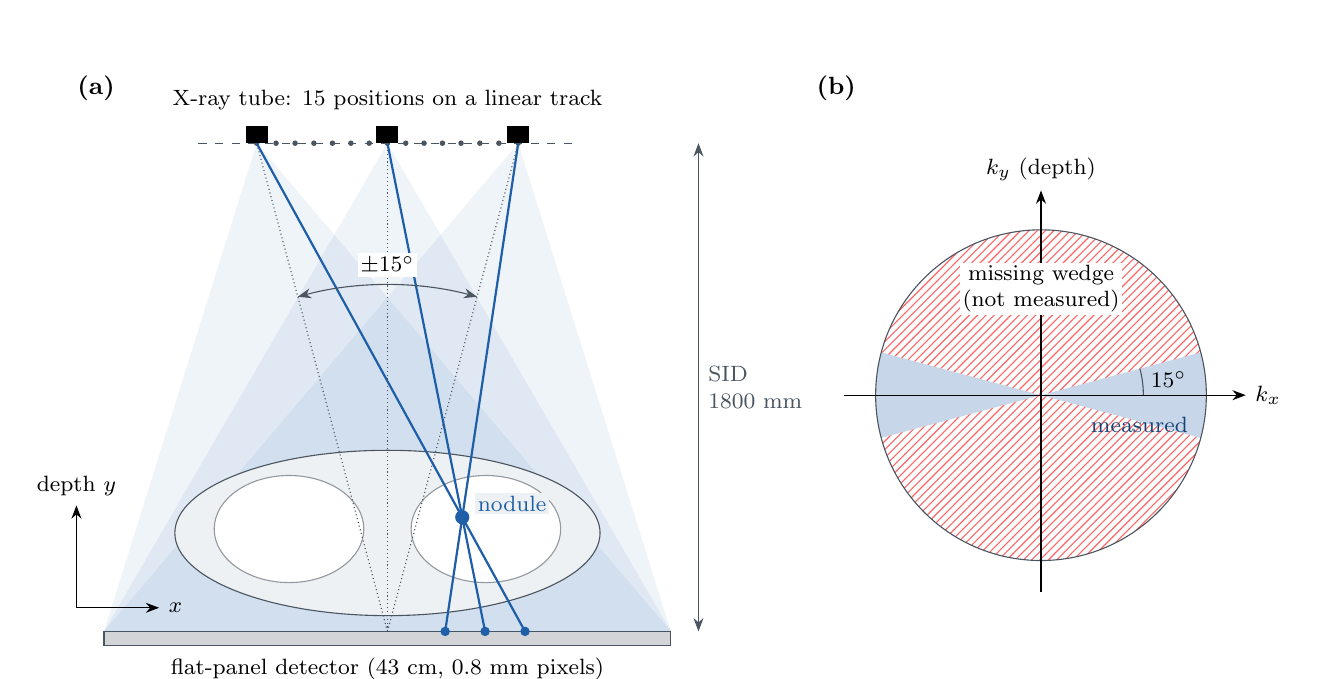
\begin{tikzpicture}[font=\footnotesize, >=Stealth]
  % ---------------- (a) geometry
  \begin{scope}
    % detector
    \fill[edge!25] (-3.6,-0.18) rectangle (3.6,0);
    \draw[edge] (-3.6,-0.18) rectangle (3.6,0);
    \node[below=1pt] at (0,-0.18) {flat-panel detector (43 cm, 0.8 mm pixels)};
    % ray fans (drawn first, behind the patient)
    \foreach \a in {-15, 0, 15} {
      \fill[uiublue, opacity=0.07] ({6.2*tan(\a)},6.2) -- (-3.6,0) -- (3.6,0) -- cycle;
    }
    % patient cross-section
    \draw[edge, fill=physics] (0,1.25) ellipse (2.7 and 1.05);
    \draw[edge!60, fill=white] (-1.25,1.3) ellipse (0.95 and 0.68);
    \draw[edge!60, fill=white] (1.25,1.3) ellipse (0.95 and 0.68);
    % source track
    \draw[edge, dashed] (-2.4,6.2) -- (2.4,6.2);
    \foreach \a in {-15,-12.857,...,15.1} {
      \fill[edge] ({6.2*tan(\a)},6.2) circle (0.035);
    }
    % rays through the nodule to the detector: the shadow moves with the tube angle
    \foreach \a in {-15, 0, 15} {
      \coordinate (S) at ({6.2*tan(\a)},6.2);
      \draw[accent, thick] (S) -- ($(S)!{6.2/(6.2-1.45)}!(0.95,1.45)$) coordinate (D);
      \fill[accent] (D) circle (0.06);
      \fill[black] (S) ++(-0.14,0) rectangle ++(0.28,0.22);
    }
    \fill[accent] (0.95,1.45) circle (0.09);
    \node[accent, right=1pt, fill=physics, inner sep=1pt] at (1.07,1.62) {nodule};
    \node[above=3pt, align=center] at (0,6.4) {X-ray tube: 15 positions on a linear track};
    % sweep angle, measured at the detector centre
    \draw[edge, densely dotted] (0,0) -- (0,6.2);
    \draw[edge, densely dotted] (0,0) -- ({6.2*tan(15)},6.2);
    \draw[edge, densely dotted] (0,0) -- ({-6.2*tan(15)},6.2);
    \draw[edge, <->] ({4.4*cos(105)},{4.4*sin(105)}) arc[start angle=105, end angle=75, radius=4.4];
    \node[fill=white, inner sep=1pt] at (0,4.65) {$\pm 15^\circ$};
    % SID dimension
    \draw[<->, edge] (3.95,0) -- (3.95,6.2) node[midway, right, align=left] {SID\\1800 mm};
    % axes
    \draw[->] (-3.95,0.3) -- (-3.95,1.6) node[above] {depth $y$};
    \draw[->] (-3.95,0.3) -- (-2.9,0.3) node[right] {$x$};
    \node[font=\small\bfseries] at (-3.7,6.9) {(a)};
  \end{scope}

  % ---------------- (b) Fourier space
  \begin{scope}[xshift=8.3cm, yshift=3.0cm]
    \def\R{2.1}
    \fill[uiublue!25] (0,0) -- (-15:\R) arc[start angle=-15, end angle=15, radius=\R] -- cycle;
    \fill[uiublue!25] (0,0) -- (165:\R) arc[start angle=165, end angle=195, radius=\R] -- cycle;
    \fill[pattern=north east lines, pattern color=red!60] (0,0) -- (15:\R) arc[start angle=15, end angle=165, radius=\R] -- cycle;
    \fill[pattern=north east lines, pattern color=red!60] (0,0) -- (195:\R) arc[start angle=195, end angle=345, radius=\R] -- cycle;
    \draw[edge] (0,0) circle (\R);
    \draw[->] (-2.5,0) -- (2.6,0) node[right] {$k_x$};
    \draw[->] (0,-2.5) -- (0,2.6) node[above] {$k_y$ (depth)};
    \node[fill=white, inner sep=1pt, align=center] at (0,1.35) {missing wedge\\(not measured)};
    \node[align=center, text=uiublue!70!black] at (1.25,-0.38) {measured};
    \draw[edge] (1.3,0) arc[start angle=0, end angle=15, radius=1.3];
    \node at (1.62,0.2) {$15^\circ$};
    \node[font=\small\bfseries] at (-2.6,3.9) {(b)};
  \end{scope}
\end{tikzpicture}
}
  \caption[DTS acquisition geometry and the missing wedge]{Chest DTS acquisition. (a) The X-ray tube moves along a linear track over $\pm15^\circ$ and the nodule's shadow shifts on the detector with the tube angle; this shift is the only depth information. (b) In Fourier space each view measures one plane, so a $\pm15^\circ$ sweep measures only a double wedge around the in-plane axis and leaves the depth frequencies unmeasured.}
  \label{fig:dts}
\end{figure}

\section{Motivation}

This project is motivated by four observations: nodules need to be followed over time, the size of nodules is uncertain when measured in 2D, follow-up using CT is costly because of radiation, access, and existing reconstruction methods are not able to produce trustworthy numbers from DTS. Our approach is guided by a 5th, computational observation.

\subsection{Clinical Importance of Nodule Follow-up}
The 5-year survival rates are 64\% for localised lung cancer, and 9\% for distant disease~\cite{who2023lung,nlst2011}. The only distinguishing feature between malignant and benign nodules is growth and the guidelines are based on ranges of volume and doubling times: $<100$, 100--300 and $\geq$300 mm$^3$; $<400$, 400--600 and $>600$ days~\cite{horeweg2014nelson,oudkerk2017eups}.

\subsection{Limits of 2D Measurement}
 Diameters measured on single slices assume a sphere. Volumes estimated from 2D measurements differ from 3D volumetry by 47--85\% on average~\cite{demargerie2018}, 2D measurements of small nodules are unreliable~\cite{revel2004twod}, and a 1~mm change in diameter is a 33\% change in volume~\cite{lee2025volumetry}. Measurement error larger than the true growth delays treatment.

\subsection{Radiation and Access}
 CT follow-up means repeated dose and requires well-equipped centres~\cite{mascalchi2017,brenner2007ct}. In Bangladesh, CT scanners are concentrated in divisional cities and large hospitals, so many patients travel long distances and pay for every follow-up scan, while digital radiography rooms, which can be upgraded to tomosynthesis, are far more widespread. DTS is cheaper, faster and much lower in dose than CT, but today it offers no trustworthy 3D measurement, so a nodule found on DTS is still sent to CT for every follow-up.

\subsection{Why Existing Reconstruction and AI Are Not Enough}
Iterative reconstruction from a \ang{30} sweep results in 3--5 times nodule extension along the depth axis in comparison to in-plane (the median was 3.5 in our measurements of LIDC nodules). The missing wedge is generative models, but a cancer-following model that creates anatomy is hazardous~\cite{bhadra2021,zhang2025pail}. Sparse view methods have been published with image quality (PSNR,SSIM) values not calibrated clinical numbers and none is developed for DTS geometry.

\subsection{Computational Motivation}
Not only what it can show, but we asked what DTS can \emph{measure}. By derivation of projection moments (\cref{sec:method}) it is shown that every DTS view measures the total excess attenuation of a nodule exactly, its depth extent, which volume needs, is about 15 times worse conditioned for a $\pm15^\circ$ sweep. A system for DTS should therefore start with a statement of \emph{mass}, then a fill depth with a learned prior that is consistent with the X-rays, and a statement of uncertainty for each of the numbers. The use of mass growth as a CT biomarker is already proven to detect growth earlier than volume~\cite{dehoop2010}.

\section{Objectives}

The objectives are stated as testable hypotheses (H1--H6); any of them could turn out false, and \cref{ch:results} reports what we found.

\begin{enumerate}[label=\textbf{O\arabic*}]
  \item \textbf{Mass-first measurement (H1).} Show, in theory and on data, that nodule mass from DTS has a smaller error than nodule volume.
  \item \textbf{Learned prior for the missing wedge (H2).} Train a conditional 3D diffusion model that, combined with physics data consistency and 3D Gaussians, reduces volume error compared with physics-only reconstruction.
  \item \textbf{Calibrated uncertainty (H3, H5).} Give every mass and volume a conformal 90\% prediction interval that reaches its nominal coverage on held-out patients, and give calibrated probabilities of the clinical size categories with coverage in every size group.
  \item \textbf{Growth (H4).} Measure growth on virtual follow-up scans and test whether mass doubling time (MDT) classifies growth more accurately than VDT.
  \item \textbf{Explainability (H6).} Show for each nodule which part of the 3D result was measured by the X-rays (seen) and which was supplied by the prior (unseen), and test whether the prior's unseen content recovers the truth rather than inventing it.
  \item \textbf{Usable system.} Deliver a click-to-3D application with a learned detector that suggests where to click, running on free or low-cost cloud hardware.
\end{enumerate}

\section{Methodology}

MedLift-3D is evaluated as a virtual clinical trial on real patient CT, because no public dataset has chest DTS together with CT ground truth. \Cref{fig:pipeline} in \cref{ch:design} shows the full pipeline.
\begin{enumerate}
  \item \textbf{Data:} 583 LIDC-IDRI patients with \num{1144} nodules of 4--30~mm marked by at least three of four radiologists~\cite{armato2011lidc,hancock2016pylidc}, split by patient 60/20/20 into training, calibration and test sets.
  \item \textbf{DTS simulation:} 15 low-dose views over $\pm15^\circ$ with Poisson noise, reconstructed by SIRT~\cite{gilbert1972sirt}.
  \item \textbf{Click and prism:} the clinician, helped by a learned detector, selects a nodule; a 64~mm column through the whole chest (the \emph{prism}) is reconstructed around it.
  \item \textbf{Diffusion prior:} a 17.4-million-parameter conditional 3D U-Net diffusion model~\cite{ho2020ddpm,song2021ddim,salimans2022v} generates eight CT-like hypotheses of the prism, each kept consistent with the X-rays by SIRT steps inside the sampler.
  \item \textbf{3D Gaussians:} each hypothesis is fitted with anisotropic 3D Gaussians~\cite{kerbl2023gs,zha2024r2}, which give the nodule's mass in closed form.
  \item \textbf{Uncertainty:} the spread of the eight hypotheses is calibrated into conformal intervals and predictive distributions on the calibration patients~\cite{vovk2022alrw,vovk2019cps,bostrom2022crepes,angelopoulos2023}.
  \item \textbf{Explanation:} each result is split into seen and unseen parts by a conjugate-gradient null-space decomposition~\cite{bhadra2021,wang2023ddnm}, and the detector is explained with input$\times$gradient saliency~\cite{shrikumar2017}.
\end{enumerate}

\section{Project Outcome}

The project generates the following three sets of outputs: a technical system that is shown to operate; a system usable by a clinician; and a research contribution.

\subsection{Technical Outcome}
An automated, step-by-step, scripted process from data download to final tables, figures and HTML report, which has been verified and passed. It includes a differentiatable DTS simulator and projector, whole-chest and prism reconstruction, a trained conditional diffusion prior and nodule detector, Gaussian measurement, conformal calibration and an explainability module, with 69 unit tests documented and with free use of cloud GPUs via a rental service and Kaggle notebooks.

\subsection{Clinical Outcome}
 A click-to-3D application that returns, in under a minute, the nodule's mass, volume, long-axis diameter and EUPS size category with calibrated probabilities, together with a virtual follow-up for growth. Every number comes with an interval instead of a single value, and a low-confidence flag tells the clinician when the DTS evidence is too weak and a CT is advisable. The tool is meant for following known nodules, the step that today requires repeated CT.

\subsection{Research Contribution}
 (i) A projection-moment argument that DTS measures mass but not depth extent; (ii) a data-consistent diffusion prior inside a DTS prism combined with Gaussian mass; (iii) calibrated, decision-level uncertainty for DTS volumetry; (iv) a truth-referenced seen/unseen test of what the prior adds. \Cref{sec:gap} states exactly what is and is not new.

\section{Organization of the Report}

\Cref{ch:background} provides the background of DTS, diffusion models, 3D Gaussians, conformal prediction and explainability, discusses related applications and research, and identifies the gap. The requirements, context and data flow diagrams, user interface, detailed method, including alternatives examined, project plan and task allocation are presented in \cref{ch:design}. \Cref{ch:results} describes the environment and tools as well as how each requirement was verified and the results of H1-H6. \Cref{ch:standards} discusses standards, issues related to society, health and safety, law, culture, ethics, environment and sustainability, costs and the complex engineering problem mapping. In \cref{ch:conclusion} the work is summarised, limitations are pointed out, future work is suggested and what has been learnt is summarised.

\chapter{Background}
\label{ch:background}

This chapter gives the background needed for the rest of the report and reviews existing applications and research. It concludes in the gap that MedLift-3D fills.

\section{Preliminaries}

This section presents the physics of X-ray projection and tomosynthesis, iterative reconstruction and null space, diffusion models, Gaussian representations and nodule mass, conformal prediction, and explainability and detection measures which are used throughout the remainder of the report.

\subsection{X-ray Projection and Digital Tomosynthesis}
 A detector pixel records the line integral of the linear attenuation coefficient $\mu$ along the ray from the source. With $I_0$ incident photons the expected count is
\begin{equation}
  \bar I = I_0 \exp\Big(-\int_{\text{ray}} \mu(\mathbf{r})\, \mathrm{d}l\Big), \qquad I \sim \mathrm{Poisson}(\bar I),
\end{equation}
so fewer photons (lower dose) mean more noise. CT values are expressed in Hounsfield units, $\mathrm{HU} = 1000\,(\mu-\mu_{\text{water}})/\mu_{\text{water}}$.

\paragraph{The missing wedge.} CT collects projections over \ang{180} or more. Chest DTS moves the tube along a short linear track, typically $\pm15^\circ$ (GE VolumeRAD) to $\pm20^\circ$ (Shimadzu SonialVision), with 15--74 views~\cite{dobbins2003dts}. By the Fourier slice theorem each view measures one plane of the object's 3D Fourier transform, so a narrow sweep leaves a wedge of depth frequencies unmeasured (\cref{fig:dts}b). Reconstructions are sharp in the coronal plane but every structure is smeared in depth.

\subsection{Iterative Reconstruction and the Null Space}
 Writing the projection operator as $A$, the measured line integrals as $\mathbf{b}$ and the volume as $\mathbf{x}$, SIRT~\cite{gilbert1972sirt,herman2009} solves $A\mathbf{x}\approx\mathbf{b}$ by repeated normalised back-projection of the residual:
\begin{equation}
  \mathbf{x}^{(k+1)} = \mathbf{x}^{(k)} + \lambda\, C A^{\top} R \big(\mathbf{b} - A\mathbf{x}^{(k)}\big),
\end{equation}
where $R$ and $C$ hold the inverse row and column sums of $A$. It is stable under noise but cannot recover anything that lies in the null space of $A$.

\paragraph{Seen and unseen parts.} Any volume splits uniquely as $\mathbf{x} = \mathbf{x}_{\text{seen}} + \mathbf{x}_{\text{unseen}}$ with $\mathbf{x}_{\text{seen}} \in \mathcal{R}(A^{\top})$ and $\mathbf{x}_{\text{unseen}} \in \mathcal{N}(A)$, i.e.\ $A\mathbf{x}_{\text{unseen}}=0$. The X-rays determine only the seen part; the unseen part of any reconstruction comes from its prior~\cite{bhadra2021,wang2023ddnm}. \Cref{fig:seen} illustrates this.

\begin{figure}[htbp]
  \centering
  \resizebox{0.82\linewidth}{!}{% Seen (range) / unseen (null-space) decomposition and what each reconstruction contributes
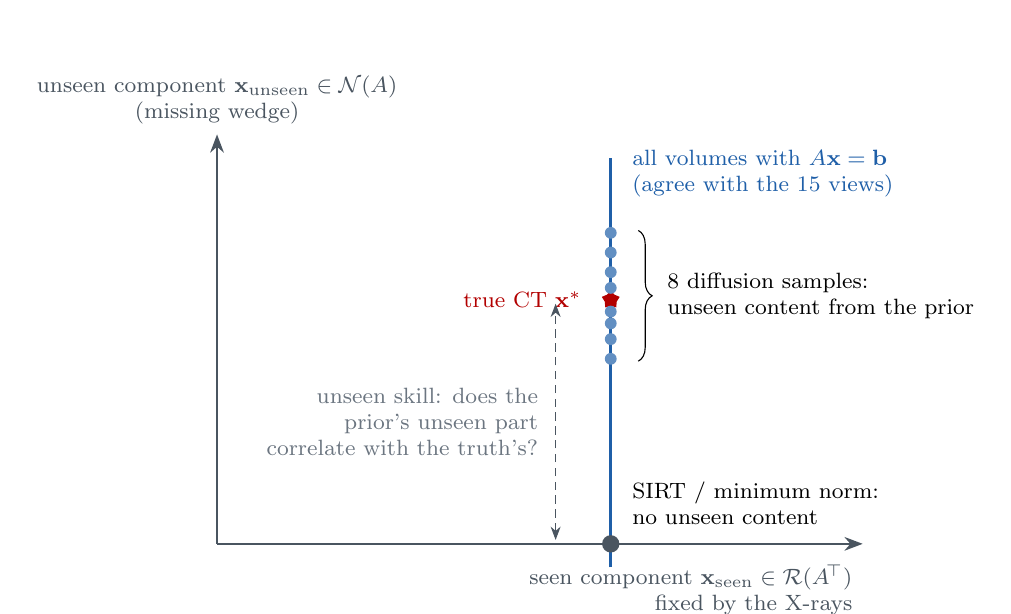
\begin{tikzpicture}[font=\footnotesize, >=Stealth]
  \draw[->, thick, edge] (0,0) -- (8.2,0) node[below=4pt, anchor=north east, align=right] {seen component $\mathbf{x}_{\mathrm{seen}} \in \mathcal{R}(A^{\!\top})$\\ fixed by the X-rays};
  \draw[->, thick, edge] (0,0) -- (0,5.2) node[above, align=center] {unseen component $\mathbf{x}_{\mathrm{unseen}} \in \mathcal{N}(A)$\\ (missing wedge)};
  % data-consistent set
  \draw[accent, very thick] (5,-0.3) -- (5,4.9);
  \node[accent, align=left, anchor=west] at (5.15,4.7) {all volumes with $A\mathbf{x} = \mathbf{b}$\\ (agree with the 15 views)};
  % SIRT / min norm
  \fill[edge] (5,0) circle (0.11);
  \node[anchor=south west, align=left] at (5.15,0.12) {SIRT / minimum norm:\\ no unseen content};
  % truth
  \node[star, star points=5, fill=red!70!black, inner sep=1.6pt] (gt) at (5,3.1) {};
  \node[anchor=east, text=red!70!black] at (4.75,3.1) {true CT $\mathbf{x}^\ast$};
  % prior samples
  \foreach \y in {2.35,2.6,2.8,2.95,3.25,3.45,3.7,3.95} { \fill[accent!70] (5,\y) circle (0.075); }
  \draw[decorate, decoration={brace, amplitude=5pt}] (5.35,3.98) -- (5.35,2.32) node[midway, right=7pt, align=left] {8 diffusion samples:\\ unseen content from the prior};
  % skill annotation
  \draw[<->, densely dashed, edge] (4.3,0.05) -- (4.3,3.05);
  \node[anchor=east, align=right, text=quiet] at (4.2,1.55) {unseen skill: does the\\ prior's unseen part\\ correlate with the truth's?};
\end{tikzpicture}
}
  \caption[Seen and unseen components of a reconstruction]{Seen (range) and unseen (null-space) components. All volumes on the vertical line agree with the measured views. SIRT returns the minimum-norm point with no unseen content; diffusion samples supply unseen content, which we test against the true CT (unseen skill, \cref{sec:method}).}
  \label{fig:seen}
\end{figure}

\subsection{Denoising Diffusion Models}
 A diffusion model learns to reverse a gradual noising process~\cite{ho2020ddpm}. With a cosine noise schedule $\bar\alpha_t$~\cite{nichol2021improved}, a noisy sample is
\begin{equation}
  \mathbf{x}_t = \sqrt{\bar\alpha_t}\,\mathbf{x}_0 + \sqrt{1-\bar\alpha_t}\,\boldsymbol\epsilon, \qquad \boldsymbol\epsilon\sim\mathcal{N}(\mathbf{0},I).
\end{equation}
We train the network to predict the velocity $\mathbf{v} = \sqrt{\bar\alpha_t}\,\boldsymbol\epsilon - \sqrt{1-\bar\alpha_t}\,\mathbf{x}_0$ (v-prediction~\cite{salimans2022v}), minimising
\begin{equation}
  \mathcal{L}(\theta) = \mathbb{E}_{\mathbf{x}_0,\mathbf{c},t,\boldsymbol\epsilon}\, \big\| \mathbf{v} - \hat{\mathbf{v}}_\theta(\mathbf{x}_t, \mathbf{c}, t)\big\|_2^2 ,
\end{equation}
where the condition $\mathbf{c}$ is the DTS reconstruction, so the model learns $p(\mathbf{x}_0\mid\mathbf{c})$. DDIM~\cite{song2021ddim} samples in tens of steps instead of a thousand, and data-consistency (DC) sampling corrects every denoised estimate with the physics so that samples agree with the measurements~\cite{chung2023dps,chung2024dds}.

\subsection{3D Gaussian Representations and Nodule Mass}
 A volume can be written as a sum of anisotropic Gaussians with centres $\boldsymbol\mu_i$, covariances $\Sigma_i = R_i S_i S_i^{\top} R_i^{\top}$ and amplitudes $a_i$~\cite{kerbl2023gs,zha2024r2}:
\begin{equation}
  f(\mathbf{r}) = \sum_i a_i \exp\!\Big(-\tfrac12(\mathbf{r}-\boldsymbol\mu_i)^{\top}\Sigma_i^{-1}(\mathbf{r}-\boldsymbol\mu_i)\Big),
  \qquad
  M = \int f = \sum_i a_i (2\pi)^{3/2} s_{i1}s_{i2}s_{i3},
  \label{eq:gaussmass}
\end{equation}
where $s_{i1},s_{i2},s_{i3}$ are the Gaussian's standard deviations. The mass is therefore closed form, and the field can be evaluated on any grid.

\paragraph{Nodule mass.} In this report mass is the nodule's excess attenuation over the surrounding lung, converted to milligrams with the CT density scale (about 0.7--0.85~mg/mm$^3$ on LIDC nodules). Mass doubling time is computed like VDT but from mass; it detects growth of part-solid nodules earlier~\cite{dehoop2010}.

\subsection{Conformal Prediction}
 Split conformal prediction~\cite{vovk2022alrw,angelopoulos2023} turns any predictor into intervals with a finite-sample guarantee: if calibration and test cases are exchangeable, a $(1-\alpha)$ interval contains the truth with probability at least $1-\alpha$. A \emph{normalised} version scales each interval by a difficulty estimate (here the spread of the diffusion hypotheses); a \emph{Mondrian} version calibrates within groups (here nodule size groups) so that coverage holds in every group; and \emph{conformal predictive systems} (CPS) return a full calibrated cumulative distribution for each case~\cite{vovk2019cps,bostrom2022crepes}, from which calibrated probabilities such as $P(V\geq 300~\text{mm}^3)$ follow. \Cref{fig:conformal} shows the procedure.

\begin{figure}[htbp]
  \centering
  \resizebox{\linewidth}{!}{% Split-conformal calibration on held-out patients and its use on a new nodule
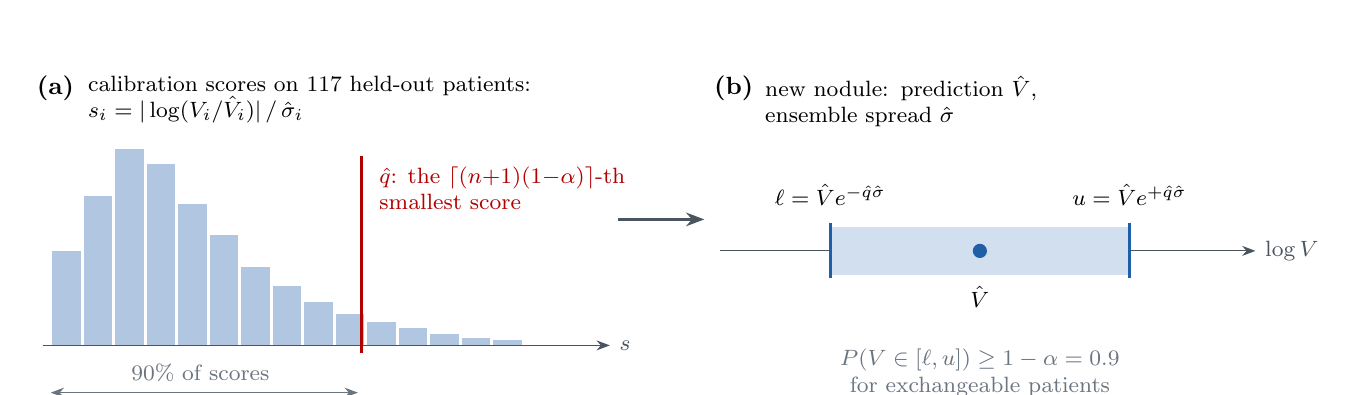
\begin{tikzpicture}[font=\footnotesize, >=Stealth]
  % (a) calibration scores
  \begin{scope}
    \node[anchor=north west, font=\small\bfseries] at (-0.2,3.55) {(a)};
    \node[anchor=north west, text width=6.8cm] at (0.45,3.55) {calibration scores on 117 held-out patients:\\ $s_i = |\log(V_i/\hat V_i)|\,/\,\hat\sigma_i$};
    \draw[->, edge] (0,0) -- (7.2,0) node[right] {$s$};
    \foreach \x/\h in {0.3/1.2,0.7/1.9,1.1/2.5,1.5/2.3,1.9/1.8,2.3/1.4,2.7/1.0,3.1/0.75,3.5/0.55,3.9/0.4,4.3/0.3,4.7/0.22,5.1/0.15,5.5/0.1,5.9/0.07} {
      \fill[accent!35] (\x-0.18,0) rectangle (\x+0.18,\h);
    }
    \draw[red!70!black, very thick] (4.05,-0.1) -- (4.05,2.4);
    \node[red!70!black, align=left, anchor=west] at (4.15,2.0) {$\hat q$: the $\lceil (n{+}1)(1{-}\alpha)\rceil$-th\\ smallest score};
    \node[text=quiet] at (2.0,-0.35) {90\% of scores};
    \draw[<->, quiet] (0.1,-0.6) -- (4.0,-0.6);
  \end{scope}
  % (b) test interval
  \begin{scope}[xshift=8.6cm]
    \node[anchor=north west, font=\small\bfseries] at (-0.2,3.55) {(b)};
    \node[anchor=north west, text width=6.5cm] at (0.45,3.55) {new nodule: prediction $\hat V$,\\ ensemble spread $\hat\sigma$};
    \draw[->, edge] (0,1.2) -- (6.8,1.2) node[right] {$\log V$};
    \fill[accent!20] (1.4,0.9) rectangle (5.2,1.5);
    \draw[accent, very thick] (1.4,0.85) -- (1.4,1.55) (5.2,0.85) -- (5.2,1.55);
    \fill[accent] (3.3,1.2) circle (0.09);
    \node[below=5pt] at (3.3,1.05) {$\hat V$};
    \node[above=3pt] at (1.4,1.55) {$\ell = \hat V e^{-\hat q\hat\sigma}$};
    \node[above=3pt] at (5.2,1.55) {$u = \hat V e^{+\hat q\hat\sigma}$};
    \node[align=center, text=quiet] at (3.3,-0.35) {$P(V \in [\ell,u]) \geq 1-\alpha = 0.9$\\ for exchangeable patients};
  \end{scope}
  \draw[->, thick, edge] (7.3,1.6) -- (8.4,1.6);
\end{tikzpicture}
}
  \caption[Split-conformal calibration]{Split-conformal calibration (schematic). (a) Normalised scores on held-out calibration patients and their $(1-\alpha)$ quantile $\hat q$. (b) The interval for a new nodule, valid for exchangeable patients without any assumption on the error distribution.}
  \label{fig:conformal}
\end{figure}

\subsection{Explainability and Detection Metrics}
 Input$\times$gradient saliency~\cite{shrikumar2017} multiplies each input voxel by the gradient of the output with respect to it, showing which voxels drove a detector's score. Detection is measured by the Competition Performance Metric (CPM), the mean sensitivity at 1/8, 1/4, 1/2, 1, 2, 4 and 8 false positives per scan~\cite{setio2017luna}.

\section{Literature Review}

The review has two parts: applications that already address parts of the problem in practice, and research on radiation and screening, nodule measurement, chest DTS, deep priors for sparse-view reconstruction, Gaussian tomography, and trustworthiness and uncertainty.

\subsection{Similar Applications}

Parts of the problem are already available in clinical practice, but the tools available do not measure nodules in 3D from DTS. The GE and Shimadzu chest DTS units generate coronal slices which radiologists read visually, and nodule size is either estimated visually or a diameter is provided in a single slice. CT nodule software, offered by scanner vendors and AI companies, segments nodules and report volumes and doubling time -- but only on CT. Detection systems like the ones compared in the LUNA16 challenge predict the locations of nodules but do not measure them. Manual segmentation is possible with general tools, like 3D Slicer, ITK-SNAP, etc., which do not carry out any learnt prior or uncertainty, while the research codes for sparse-view reconstruction generate the whole volumes for CT geometry and report only the image quality. These applications are summarised in \cref{tab:similar} and each has a drawback for our problem.

\begin{table}[!htbp]
\centering\small
\caption{Applications similar to MedLift-3D.}
\label{tab:similar}
\begin{tabularx}{\linewidth}{>{\raggedright\arraybackslash}p{3.6cm} >{\raggedright\arraybackslash}X >{\raggedright\arraybackslash}X}
\toprule
Application & What it does & What it lacks for our problem \\
\midrule
Chest DTS units (GE VolumeRAD, Shimadzu SonialVision) & Acquire and reconstruct DTS slices for reading & No 3D nodule measurement; depth smear left to the reader \\
CT nodule volumetry software (vendor lung packages, AI nodule tools) & Detect and segment nodules on CT, report volume and VDT & Requires CT at every follow-up; no DTS support \\
CT computer-aided detection (LUNA16-style)~\cite{setio2017luna} & Suggest nodule locations on CT & Detection only; no measurement or uncertainty \\
3D Slicer, ITK-SNAP & Viewing and manual segmentation & No learned prior, no calibrated numbers \\
Research sparse-view reconstruction codes (R$^2$-Gaussian, 3DGR-CT)~\cite{zha2024r2,li2025gr} & Reconstruct whole volumes from few views & CT geometry, image metrics only, no clinical numbers \\
\bottomrule
\end{tabularx}
\end{table}

\subsection{Related Research}

\paragraph{Radiation and screening.} Mascalchi and Sali~\cite{mascalchi2017} reviewed the cumulative dose of low-dose CT screening (9.3--13.0~mSv over ten years) and argued for ALARA and ultra-low-dose methods; Rampinelli et al.~\cite{rampinelli2017} estimated the cancer risk from screening and follow-up CT.

\paragraph{3D measurement of nodules.} Lee~\cite{lee2025volumetry} and de Margerie-Mellon et al.~\cite{demargerie2018} showed that volumetry is more reproducible than diameters but varies between software, and Revel et al.~\cite{revel2004twod} showed that 2D measurements of small nodules are unreliable. NELSON~\cite{horeweg2014nelson} and the European position statement~\cite{oudkerk2017eups} define the volume and VDT categories we use. De Hoop et al.~\cite{dehoop2010} showed that mass detects growth of ground-glass nodules earlier than volume or diameter.

\paragraph{Chest DTS.} Vikgren et al.~\cite{vikgren2008} found that DTS detected about three times more nodules than chest radiography, and Dobbins and Godfrey~\cite{dobbins2003dts} described the depth-resolution limit set by the sweep angle. DTS studies measure nodules in 2D or by reader judgement.

\paragraph{Sparse-view CT with deep priors.} Score-based and diffusion models have been applied in the sinogram domain~\cite{guan2024sino}, with wavelet decompositions~\cite{xu2024sword,wu2024wavelet}, for spectral CT~\cite{liu2024spectral} and zero-shot with variational solvers~\cite{he2025vss}; DPS and DDS add data consistency to sampling~\cite{chung2023dps,chung2024dds}, and foundation models learn lung CT priors from \num{100000} scans~\cite{wang2025lctfound}. Classical iterative reconstruction~\cite{herman2009} and compressed sensing~\cite{candes2006} suppress noise but over-smooth fine detail, and implicit neural fields~\cite{mildenhall2020nerf} are slow per patient. Lighter physics-conditioned diffusion~\cite{vavekanand2025}, deep image prior with ADMM~\cite{chang2025dip}, mixed priors for metal artifacts~\cite{jiang2025mixed}, learned view sampling~\cite{yang2025sampling} and unsupervised low-dose denoising~\cite{jeon2023mmnet} address other parts of the problem. All of these report image quality on CT volumes; none produces a calibrated clinical measurement or uses DTS geometry.

\paragraph{3D Gaussians in tomography.} 3DGR-CT~\cite{li2025gr} and R$^2$-Gaussian~\cite{zha2024r2} reconstruct sparse-view CT with Gaussians, and spatiotemporal Gaussians handle motion~\cite{xie2025pmf,liu2025fmgs}. They use Gaussians for speed and quality, not for closed-form mass, and have no learned prior for the missing wedge.

\paragraph{Trustworthiness and uncertainty.} Bhadra et al.~\cite{bhadra2021} defined hallucinations through the null space of the imaging operator, DDNM~\cite{wang2023ddnm} uses a range--null-space decomposition inside diffusion sampling, and Zhang et al.~\cite{zhang2025pail} used uncertainty estimates to suppress artifacts in limited-data CT. Conformal predictive systems are available in the open-source crepes library~\cite{bostrom2022crepes} but have not been applied to imaging biomarkers from DTS.

\begin{table}[!htbp]
\centering\small
\caption{Summary of the most related research.}
\label{tab:related}
\begin{tabularx}{\linewidth}{>{\raggedright\arraybackslash}p{2.6cm} >{\raggedright\arraybackslash}p{2.6cm} >{\raggedright\arraybackslash}X >{\raggedright\arraybackslash}X}
\toprule
Work & Method & Key finding & Gap for DTS nodule measurement \\
\midrule
Li et al.~\cite{li2025gr} & FBP-guided 3D Gaussians & Faster than neural fields & Whole-volume CT; no prior; no measurement \\
Zha et al.~\cite{zha2024r2} & Radiative Gaussian splatting & Accurate volume integration & No learned prior; no uncertainty \\
Guan et al.~\cite{guan2024sino} & Sinogram-domain diffusion & Handles varying sparsity & 2D; no 3D consistency \\
He et al.~\cite{he2025vss} & Zero-shot variational score solver & No paired data needed & Heavy compute; image metrics only \\
Chung et al.~\cite{chung2023dps,chung2024dds} & DPS / DDS sampling & Measurement-consistent samples & Not for DTS; not calibrated \\
Wang and Guo~\cite{wang2025lctfound} & Lung CT foundation model & Strong transfer & CT only \\
Bhadra et al.~\cite{bhadra2021} & Null-space hallucination maps & Formal definition of hallucination & No truth-referenced skill per nodule \\
Zhang et al.~\cite{zhang2025pail} & Progressive artifact learning & Fewer false structures & Uncertainty not calibrated \\
de Hoop et al.~\cite{dehoop2010} & Nodule mass on CT & Mass detects growth earlier & CT only \\
Bostr\"om~\cite{bostrom2022crepes} & Conformal predictive systems & Valid CDFs for any regressor & Not applied to imaging biomarkers \\
\bottomrule
\end{tabularx}
\end{table}

\section{Gap Analysis}
\label{sec:gap}

The review shows four gaps. First, DTS research stops at 2D detection and size; no work argues from the projection physics which 3D quantity DTS can measure. Second, generative sparse-view methods target whole CT volumes and image metrics, not a clinical number for one nodule, and none is built for the DTS sweep. Third, Gaussian tomography uses Gaussians for speed, not for closed-form mass. Fourth, reconstruction uncertainty is usually raw variance, which is not calibrated, and explanations of what a prior invented are not checked against the truth. \Cref{tab:gap} compares the closest works.

\begin{table}[!htbp]
\centering\small
\caption{Domain comparison: \cmark\ addressed, \xmark\ not addressed, $\circ$ partially.}
\label{tab:gap}
\begin{adjustbox}{max width=\linewidth}
\begin{tabular}{l ccccccc}
\toprule
Work & \makecell{DTS\\geometry} & \makecell{Learned\\prior} & \makecell{Data\\consistency} & \makecell{Gaussian\\mass} & \makecell{Clinical\\biomarker} & \makecell{Calibrated\\uncertainty} & \makecell{Seen/unseen\\explanation} \\
\midrule
Li et al.~\cite{li2025gr} & \xmark & \xmark & \cmark & \xmark & \xmark & \xmark & \xmark \\
Zha et al.~\cite{zha2024r2} & \xmark & \xmark & \cmark & \xmark & \xmark & \xmark & \xmark \\
He et al.~\cite{he2025vss} & \xmark & \cmark & \cmark & \xmark & \xmark & \xmark & \xmark \\
Chung et al.~\cite{chung2023dps} & \xmark & \cmark & \cmark & \xmark & \xmark & \xmark & \xmark \\
Zhang et al.~\cite{zhang2025pail} & \xmark & \cmark & \cmark & \xmark & \xmark & $\circ$ & \xmark \\
Bhadra et al.~\cite{bhadra2021} & \xmark & \xmark & -- & \xmark & \xmark & \xmark & \cmark \\
de Hoop et al.~\cite{dehoop2010} & \xmark & \xmark & -- & \xmark & \cmark & \xmark & \xmark \\
\midrule
\textbf{MedLift-3D} & \cmark & \cmark & \cmark & \cmark & \cmark & \cmark & \cmark \\
\bottomrule
\end{tabular}
\end{adjustbox}
\end{table}

\paragraph{What we do not claim.} 3D Gaussians in medical imaging, uncertainty for Gaussian reconstructions, conformal prediction in CT and for lung nodules, null-space hallucination analysis and saliency maps all exist already. Our contribution is their combination for DTS nodule measurement, the mass-first argument, and a calibrated, truth-checked evaluation.

\section{Summary}

DTS is low-dose and affordable but blind in depth, and existing AI reconstruction neither respects which quantities DTS can measure nor states how far its numbers can be trusted. MedLift-3D addresses this gap by measuring mass first, filling depth with a data-consistent diffusion prior, calibrating every number with conformal methods, and explaining what was measured and what was supplied by the prior. \Cref{ch:design} turns this into requirements and a design.

\chapter{Project Design}
\label{ch:design}

This chapter turns the problem into requirements, models the system with context, data flow and decomposition diagrams, and explains the method together with the alternatives we rejected. It ends with the project plan and task allocation.

\section{Requirement Analysis}

\paragraph{Requirements elicitation.} Requirements were gathered from four sources: (i) the clinical guidelines that radiologists follow for nodules, namely the EUPS volume categories and the NELSON doubling-time categories~\cite{oudkerk2017eups,horeweg2014nelson}; (ii) meetings with our supervisor; (iii) the published limits of DTS and sparse-view reconstruction (\cref{ch:background}); and (iv) the constraints of a student project: public data only, no clinical scanner, limited computing resources and a fixed deadline. \Cref{tab:stakeholders} lists the stakeholders and their needs.

\begin{table}[!htbp]
\centering\small
\caption{Stakeholders and their needs.}
\label{tab:stakeholders}
\begin{tabularx}{\linewidth}{>{\raggedright\arraybackslash}p{2.8cm} >{\raggedright\arraybackslash}X >{\raggedright\arraybackslash}X}
\toprule
Stakeholder & Need & How MedLift-3D answers it \\
\midrule
Radiologist & A 3D size and growth rate from a low-dose exam, and to know when not to trust it & Mass, volume, category and doubling time, each with a calibrated interval and a low-confidence flag \\
Patient & Less radiation and cost per follow-up & DTS at about 0.1~mSv instead of CT \\
Low-resource hospital & Affordable equipment and software & DTS hardware; software runs on a single free or rented GPU \\
Examiner / researcher & Claims that can be checked & Every step ends in PASS/FAIL checks; test patients never used for tuning \\
\bottomrule
\end{tabularx}
\end{table}

\paragraph{Requirements analysis and negotiation.} Several requirements conflict; \cref{tab:conflicts} records how each conflict was resolved.

\begin{table}[!htbp]
\centering\small
\caption{Conflicting requirements and their resolution.}
\label{tab:conflicts}
\begin{tabularx}{\linewidth}{>{\raggedright\arraybackslash}p{3.4cm} >{\raggedright\arraybackslash}X >{\raggedright\arraybackslash}X}
\toprule
Conflict & Decision & Rationale \\
\midrule
Low dose vs accuracy & Simulate $I_0 = 2\times10^4$ photons per pixel and view (about 1/20--1/40 of clinical DTS dose) & Conservative: a method that works at this dose works at clinical dose \\
Clinical view count (60--74) vs compute & 15 views at equal total dose & Measured: the view count barely changes depth smear at equal dose (5.13 vs 5.34) \\
Fill the missing wedge vs never invent anatomy & Diffusion prior with X-ray data consistency, plus seen/unseen explanation & Every hypothesis agrees with the X-rays; what the prior adds is shown and tested \\
Single number vs honest uncertainty & Eight hypotheses + conformal calibration & Raw spread is not calibrated; conformal intervals have a coverage guarantee \\
Whole-volume accuracy vs GPU memory & Reconstruct only a 64~mm prism through the chest at the click & Keeps each ray's full path (a small box gave 73\% error) at $64{\times}128{\times}64$ voxels \\
Automatic detection vs false positives & The detector only suggests; the clinician clicks & The clinician stays in control; missed nodules can still be measured \\
\bottomrule
\end{tabularx}
\end{table}

\subsection{Functional and Nonfunctional Requirements}

Functional requirements state what the system must do, from loading the data to producing the report; nonfunctional requirements state the qualities it must have: speed, cost, reproducibility, validity, safety, usability, portability and privacy. Each requirement has a measurable acceptance criterion and the pipeline step that checks it (\cref{tab:fr,tab:nfr}). The criteria were chosen so that a step script can check them automatically, which makes the verification in \cref{ch:results} independent of anyone's judgement; \cref{tab:verify} reports the result for every row.

{\small
\begin{longtable}{>{\raggedright\arraybackslash}p{1.1cm} >{\raggedright\arraybackslash}p{5.6cm} >{\raggedright\arraybackslash}p{5.0cm} >{\raggedright\arraybackslash}p{1.6cm}}
\caption{Functional requirements.}\label{tab:fr}\\
\toprule
ID & Requirement & Acceptance criterion & Checked by \\
\midrule
\endfirsthead
\toprule
ID & Requirement & Acceptance criterion & Checked by \\
\midrule
\endhead
FR-01 & Load LIDC-IDRI CT and radiologist annotations; build a consensus mask ($\geq$50\% of readers); split by patient into train/cal/test & DICOM and pylidc slice positions agree; splits disjoint & Steps 02--04 \\
FR-02 & Simulate low-dose DTS: 15 views, $\pm15^\circ$, SID 1800~mm, 43~cm panel, Poisson noise & Detector integral equals object mass within 0.1\% in every view & Steps 01, 05 \\
FR-03 & Reconstruct the whole chest with SIRT, confined in depth to the patient & Residual below 0.9 of its start; missing wedge visible (depth/in-plane $>1.3$) & Step 06 \\
FR-04 & Suggest nodule candidates with a learned 3D detector & Test CPM higher than a training-free baseline & Step 14 \\
FR-05 & Reconstruct a 64~mm prism around a click & Prism keeps the column's attenuation (ratio $\approx 1$) & Step 07 \\
FR-06 & Generate eight X-ray-consistent CT hypotheses with the diffusion prior & Nodule-box PSNR of samples above the physics-only input on held-out pairs & Steps 08, 15 \\
FR-07 & Fit 3D Gaussians; measure mass, volume, 2D diameter and EUPS category & Finite values; failures reported, not hidden & Step 09 \\
FR-08 & Calibrate 90\% intervals and category probabilities & Test coverage $90\pm3\%$; Brier score below the raw ensemble vote & Steps 10, 16 \\
FR-09 & Measure growth on virtual follow-ups (VDT, MDT, NELSON categories) & Doubling-time error and category accuracy reported & Step 11 \\
FR-10 & Explain each result: seen/unseen split, detector saliency, error drivers & Tables and figures produced on test nodules & Step 17 \\
FR-11 & Interactive click-to-3D application and HTML report of all results & Demo self-test passes; report lists every check & Steps 12, 18 \\
\bottomrule
\end{longtable}
}

\begin{table}[!htbp]
\centering\small
\caption{Nonfunctional requirements.}
\label{tab:nfr}
\begin{tabularx}{\linewidth}{>{\raggedright\arraybackslash}p{3.2cm} >{\raggedright\arraybackslash}X >{\raggedright\arraybackslash}X}
\toprule
ID & Requirement & Acceptance criterion \\
\midrule
NFR-01 Performance & One click gives a result quickly & $\leq 60$~s per nodule on one GPU \\
NFR-02 Compute & The study and the application run on modest hardware & One GPU for the study; free GPU for the application \\
NFR-03 Reproducibility & Same input, same output; checkable steps & Fixed seed, one configuration file, PASS/FAIL checks, unit tests \\
NFR-04 Validity & No optimistic bias & Test patients unused for training or tuning; simulation and reconstruction on different grids \\
NFR-05 Safety & Never report a bare number & Every number has an interval; low-confidence flag when fewer than half of the hypotheses find the nodule or the spread exceeds $10\times$ \\
NFR-06 Usability & Usable by a clinician without coding & Browser interface, one click per nodule \\
NFR-07 Portability & Runs on common hardware & CPU smoke test; GPU with $\geq 24$~GB for training \\
NFR-08 Privacy & No identifiable patient data & Only de-identified public TCIA data \\
\bottomrule
\end{tabularx}
\end{table}

\subsection{Context Diagram}

The context diagram (\cref{fig:context}) depicts MedLift-3D as a single process with its external entities. The clinician is the only actor during run time: they send a case, a click and a depth and they receive the measurement report. The TCIA archive provides CT scans with the annotations from the radiologists and the cloud GPU provider performs the training and evaluation jobs and returns trained models and result, which are necessary only to build and evaluate the system, but not to use it.

\begin{figure}[htbp]
  \centering
  \resizebox{0.92\linewidth}{!}{% Context diagram (DFD level 0), Gane--Sarson notation
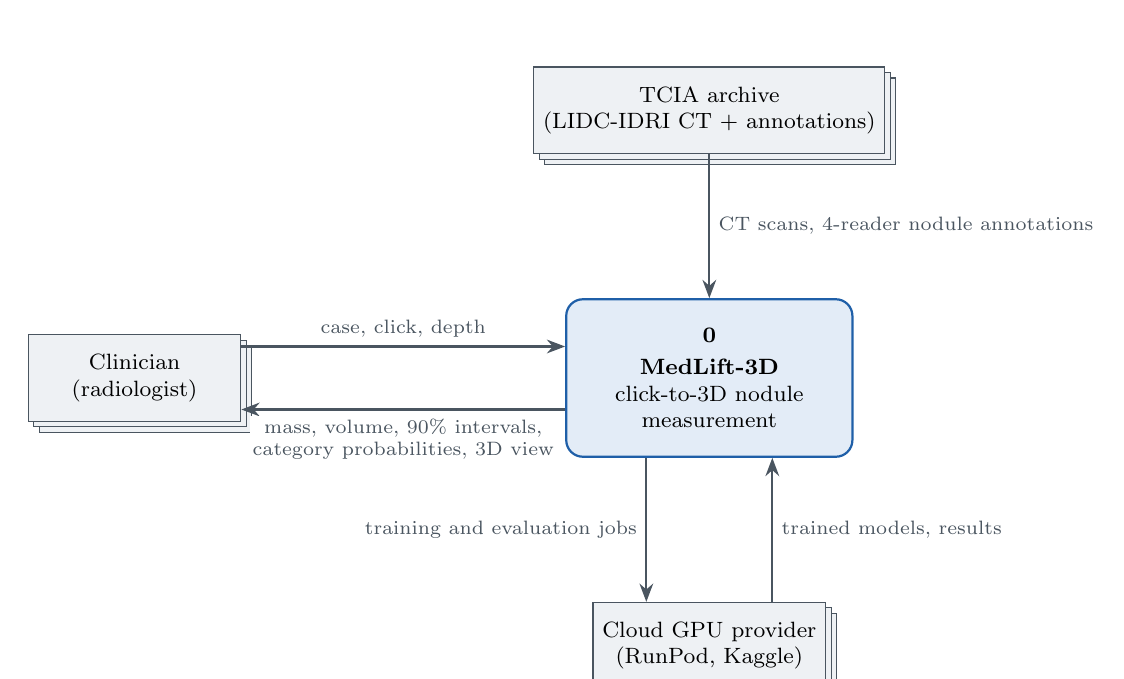
\begin{tikzpicture}
  \node[mainproc, minimum width=3.6cm, minimum height=2.0cm, text width=3.4cm] (sys) at (0,0)
       {\textbf{0}\\[2pt] \textbf{MedLift-3D}\\ click-to-3D nodule measurement};
  \node[entity] (clin) at (-7.3,0) {Clinician\\ (radiologist)};
  \node[entity] (tcia) at (0,3.4) {TCIA archive\\ (LIDC-IDRI CT + annotations)};
  \node[entity] (gpu)  at (0,-3.4) {Cloud GPU provider\\ (RunPod, Kaggle)};

  \draw[flow] ([yshift=4mm]clin.east) -- node[flowlbl, above=2pt] {case, click, depth} ([yshift=4mm]sys.west);
  \draw[flow] ([yshift=-4mm]sys.west) -- node[flowlbl, below=2pt] {mass, volume, 90\% intervals,\\ category probabilities, 3D view} ([yshift=-4mm]clin.east);
  \draw[flow] (tcia.south) -- node[flowlbl, right=2pt] {CT scans, 4-reader nodule annotations} (sys.north);
  \draw[flow] ([xshift=-8mm]sys.south) -- node[flowlbl, left=2pt] {training and evaluation jobs} ([xshift=-8mm]gpu.north);
  \draw[flow] ([xshift=8mm]gpu.north) -- node[flowlbl, right=2pt] {trained models, results} ([xshift=8mm]sys.south);
\end{tikzpicture}
}
  \caption{Context diagram (DFD level 0) in Gane--Sarson notation.}
  \label{fig:context}
\end{figure}

\subsection{Data Flow Diagram Level 1}

The level-1 DFD (\cref{fig:dfd1}) breaks down the system into eight processes and four data stores. The top row is run once for building the cases, training the models and calibrating, the second row is run every click and reads all four stores. The functional decomposition, entity-relationship model and the data dictionary are provided in \cref{sec:method}.

\begin{figure}[htbp]
  \centering
  \resizebox{\linewidth}{!}{% Data flow diagram level 1, Gane--Sarson notation
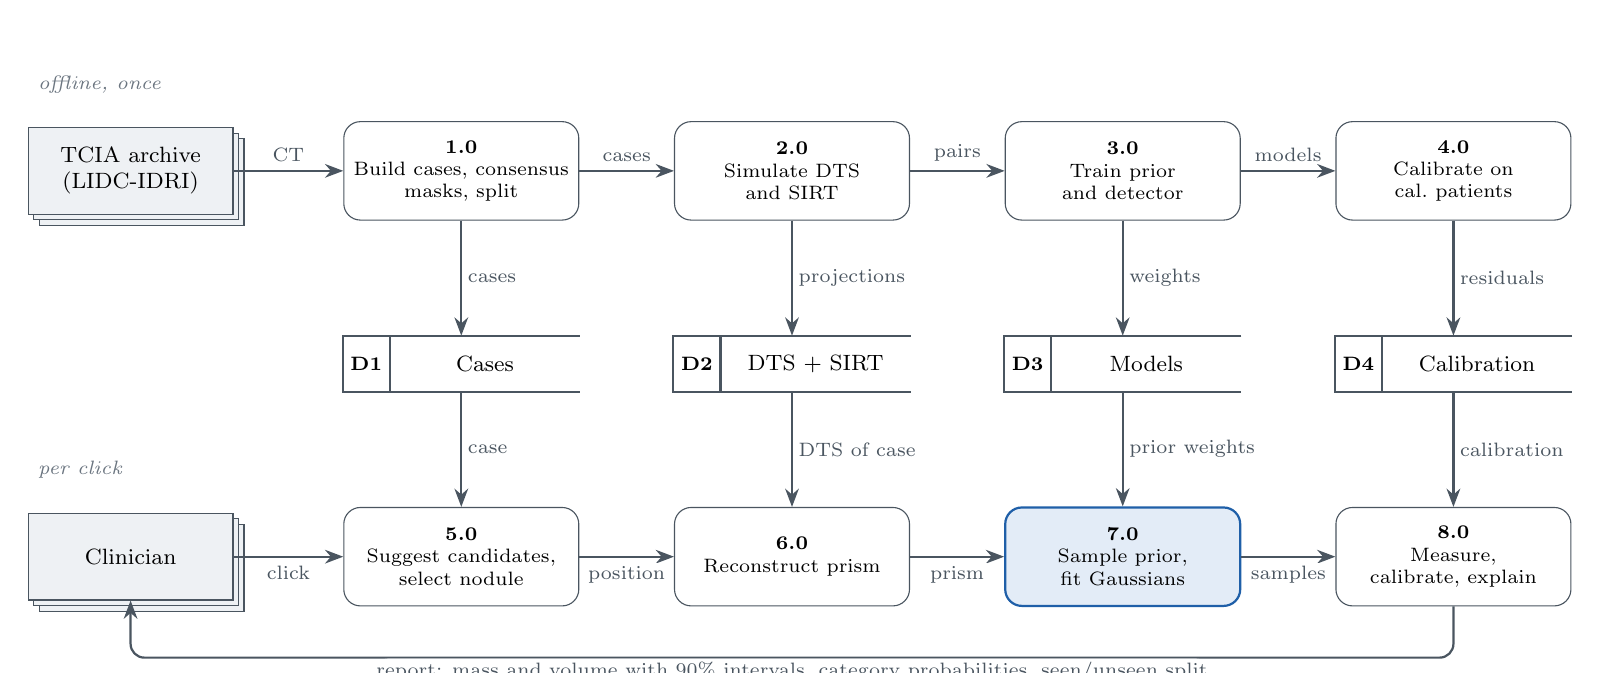
\begin{tikzpicture}[process/.append style={font=\scriptsize, text width=2.75cm, minimum width=2.95cm}, mainproc/.append style={font=\scriptsize, text width=2.75cm, minimum width=2.95cm}]
  \def\cA{0}\def\cB{4.2}\def\cC{8.4}\def\cD{12.6}\def\cE{16.8}
  \def\rTop{4.9}\def\rMid{2.45}\def\rBot{0}
  % offline row
  \node[entity, minimum width=2.6cm] (tcia) at (\cA,\rTop) {TCIA archive\\ (LIDC-IDRI)};
  \node[process] (p1) at (\cB,\rTop) {\textbf{1.0}\\ Build cases, consensus masks, split};
  \node[process] (p2) at (\cC,\rTop) {\textbf{2.0}\\ Simulate DTS and SIRT};
  \node[process] (p3) at (\cD,\rTop) {\textbf{3.0}\\ Train prior and detector};
  \node[process] (p4) at (\cE,\rTop) {\textbf{4.0}\\ Calibrate on cal.\ patients};
  % stores
  \datastore{d1}{(\cB,\rMid)}{D1}{Cases}
  \datastore{d2}{(\cC,\rMid)}{D2}{DTS + SIRT}
  \datastore{d3}{(\cD,\rMid)}{D3}{Models}
  \datastore{d4}{(\cE,\rMid)}{D4}{Calibration}
  % per-click row
  \node[entity, minimum width=2.6cm] (clin) at (\cA,\rBot) {Clinician};
  \node[process] (p5) at (\cB,\rBot) {\textbf{5.0}\\ Suggest candidates, select nodule};
  \node[process] (p6) at (\cC,\rBot) {\textbf{6.0}\\ Reconstruct prism};
  \node[mainproc] (p7) at (\cD,\rBot) {\textbf{7.0}\\ Sample prior, fit Gaussians};
  \node[process] (p8) at (\cE,\rBot) {\textbf{8.0}\\ Measure, calibrate, explain};

  \foreach \a/\b/\t in {tcia/p1/{CT}, p1/p2/{cases}, p2/p3/{pairs}, p3/p4/{models}} {
    \draw[flow] (\a) -- node[flowlbl, above=2pt] {\t} (\b);
  }
  \foreach \a/\b/\t in {clin/p5/{click}, p5/p6/{position}, p6/p7/{prism}, p7/p8/{samples}} {
    \draw[flow] (\a) -- node[flowlbl, below=2pt] {\t} (\b);
  }
  \foreach \p/\d/\t in {p1/d1/{cases}, p2/d2/{projections}, p3/d3/{weights}, p4/d4/{residuals}} {
    \draw[flow] (\p) -- node[flowlbl, right=1pt] {\t} (\d);
  }
  \foreach \d/\p/\t in {d1/p5/{case}, d2/p6/{DTS of case}, d3/p7/{prior weights}, d4/p8/{calibration}} {
    \draw[flow] (\d) -- node[flowlbl, right=1pt] {\t} (\p);
  }
  \draw[flow, rounded corners=5pt] (p8.south) -- ++(0,-0.65) -| node[flowlbl, pos=0.25, below] {report: mass and volume with 90\% intervals, category probabilities, seen/unseen split} (clin.south);
  \node[font=\scriptsize\itshape, text=quiet, anchor=west] at (-1.3,6.0) {offline, once};
  \node[font=\scriptsize\itshape, text=quiet, anchor=west] at (-1.3,1.1) {per click};
\end{tikzpicture}
}
  \caption{Data flow diagram level 1 (offline processes 1.0--4.0, per-click processes 5.0--8.0, data stores D1--D4).}
  \label{fig:dfd1}
\end{figure}





\subsection{UI Design}

The interface is a web-based application built on a single action, which is to click on the nodule (\cref{fig:ui}). The numbered parts are: (1) case and method selection; (2) the coronal DTS slice, with detector suggestions, annotated nodules (for evaluation) and with the click; (3) the depth slider, which provides the third coordinate; (4) the measurement report with mass and volume intervals, the EUPS category probabilities and the low-confidence flag; (5) a 3D view of the nodule and the prism input with its eight samples; and (6) a virtual follow-up with VDT and MDT.

\begin{figure}[htbp]
  \centering
  \resizebox{\linewidth}{!}{% User interface wireframe of the click-to-3D demo (Gradio)
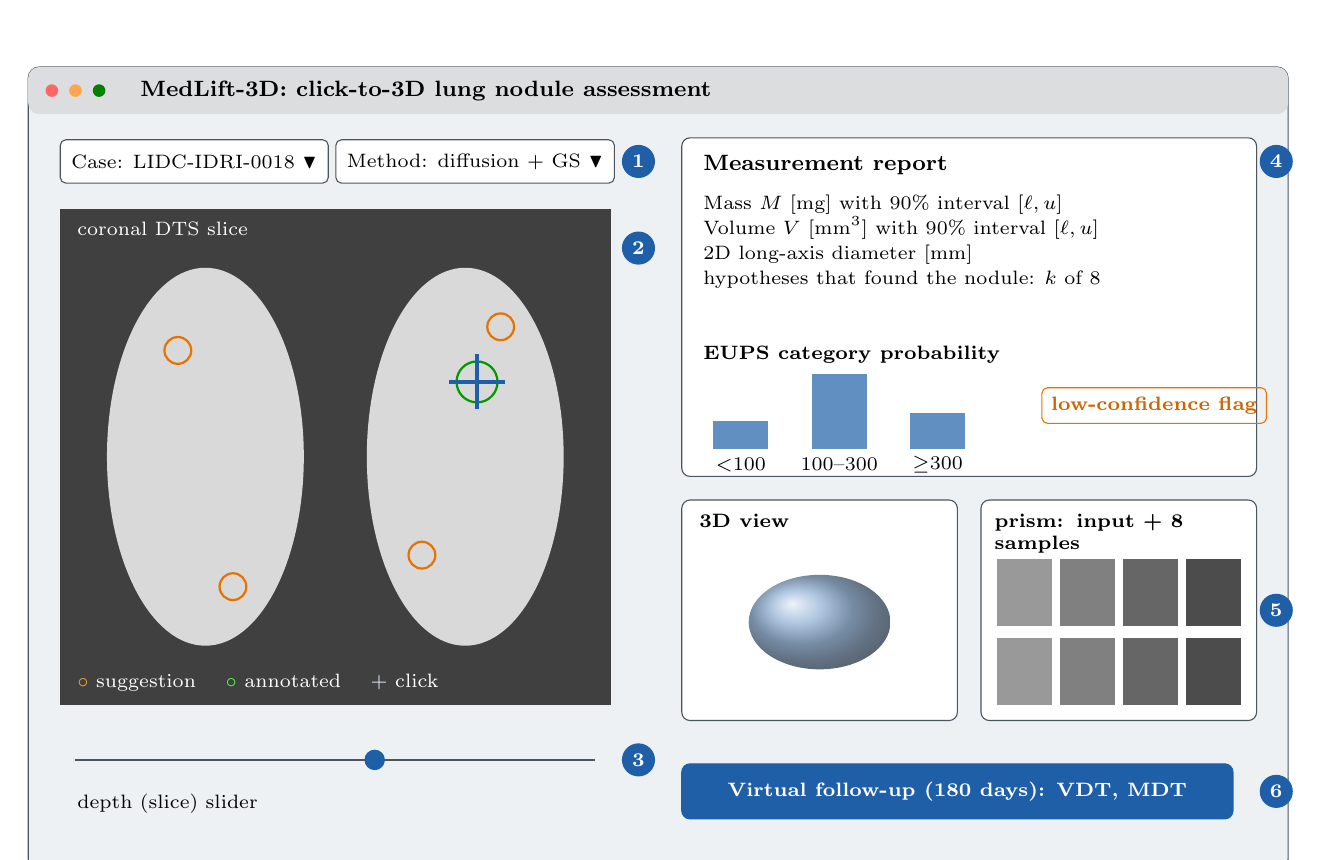
\begin{tikzpicture}[font=\footnotesize,
    ctl/.style={draw=edge, fill=white, rounded corners=2pt, minimum height=0.55cm, anchor=west, inner xsep=4pt, font=\scriptsize},
    call/.style={circle, fill=accent, text=white, font=\scriptsize\bfseries, inner sep=1pt, minimum size=0.42cm}]
  % browser frame
  \draw[edge, fill=physics, rounded corners=4pt] (0,0) rectangle (16,10.2);
  \fill[edge!20, rounded corners=4pt] (0,9.6) rectangle (16,10.2);
  \foreach \x/\c in {0.3/red!60, 0.6/orange!70, 0.9/green!50!black} { \fill[\c] (\x,9.9) circle (0.08); }
  \node[anchor=west, font=\footnotesize\bfseries] at (1.3,9.9) {MedLift-3D: click-to-3D lung nodule assessment};
  % left panel
  \node[ctl] at (0.4,9.0) {Case: LIDC-IDRI-0018 $\blacktriangledown$};
  \node[ctl] at (3.9,9.0) {Method: diffusion + GS $\blacktriangledown$};
  \node[call] at (7.75,9.0) {1};
  \fill[black!75] (0.4,2.1) rectangle (7.4,8.4);
  \fill[black!15] (2.25,5.25) ellipse (1.25 and 2.4);
  \fill[black!15] (5.55,5.25) ellipse (1.25 and 2.4);
  \foreach \p in {(1.9,6.6),(5.0,4.0),(2.6,3.6),(6.0,6.9)} { \draw[orange!90!black, thick] \p circle (0.17); }
  \draw[green!60!black, thick] (5.7,6.2) circle (0.26);
  \draw[accent, very thick] (5.7,5.85) -- ++(0,0.7) (5.35,6.2) -- ++(0.7,0);
  \node[call] at (7.75,7.9) {2};
  \node[anchor=north west, font=\scriptsize, text=white] at (0.5,8.35) {coronal DTS slice};
  \node[anchor=south west, font=\scriptsize, text=white, align=left] at (0.5,2.15) {\textcolor{orange!80}{$\circ$} suggestion \quad \textcolor{green!70}{$\circ$} annotated \quad \textcolor{accentlight}{$+$} click};
  \draw[edge, thick] (0.6,1.4) -- (7.2,1.4);
  \fill[accent] (4.4,1.4) circle (0.13);
  \node[anchor=west, font=\scriptsize] at (0.5,0.85) {depth (slice) slider};
  \node[call] at (7.75,1.4) {3};
  % right panel: report
  \draw[edge, fill=white, rounded corners=3pt] (8.3,5.0) rectangle (15.6,9.3);
  \node[anchor=north west, font=\footnotesize\bfseries] at (8.45,9.2) {Measurement report};
  \node[anchor=north west, align=left, font=\scriptsize] at (8.45,8.7)
     {Mass $M$ [mg] with 90\% interval $[\ell, u]$\\[1pt]
      Volume $V$ [mm$^3$] with 90\% interval $[\ell, u]$\\[1pt]
      2D long-axis diameter [mm]\\[1pt]
      hypotheses that found the nodule: $k$ of 8};
  \node[anchor=west, font=\scriptsize\bfseries] at (8.45,6.55) {EUPS category probability};
  \foreach \i/\h/\t in {0/0.35/{$<$100}, 1/0.95/{100--300}, 2/0.45/{$\geq$300}} {
    \fill[accent!70] ({8.7+1.25*\i},5.35) rectangle ++(0.7,\h);
    \node[font=\scriptsize] at ({9.05+1.25*\i},5.15) {\t};
  }
  \node[draw=orange!90!black, text=orange!80!black, font=\scriptsize\bfseries, rounded corners=2pt] at (14.3,5.9) {low-confidence flag};
  \node[call] at (15.85,9.0) {4};
  % 3D view and prism strip
  \draw[edge, fill=white, rounded corners=3pt] (8.3,1.9) rectangle (11.8,4.7);
  \node[anchor=north west, font=\scriptsize\bfseries] at (8.4,4.65) {3D view};
  \shade[ball color=accent!60, opacity=0.8] (10.05,3.15) ellipse (0.9 and 0.6);
  \draw[edge, fill=white, rounded corners=3pt] (12.1,1.9) rectangle (15.6,4.7);
  \node[anchor=north west, font=\scriptsize\bfseries, text width=3.2cm] at (12.15,4.65) {prism: input + 8 samples};
  \foreach \i in {0,...,3} { \foreach \j in {0,1} { \fill[black!\the\numexpr 40+10*\i\relax] ({12.3+0.8*\i},{2.1+1.0*\j}) rectangle ++(0.7,0.85); } }
  \node[call] at (15.85,3.3) {5};
  % follow-up button
  \node[draw=accent, fill=accent, text=white, rounded corners=3pt, minimum width=7.0cm, minimum height=0.7cm, font=\scriptsize\bfseries] at (11.8,1.0) {Virtual follow-up (180 days): VDT, MDT};
  \node[call] at (15.85,1.0) {6};
\end{tikzpicture}
}
  \caption{User interface design of the click-to-3D application.}
  \label{fig:ui}
\end{figure}

\section{Detailed Methodology and Design}
\label{sec:method}

This section decomposes the system into its functions and data, derives what DTS can measure, and describes the proposed architecture, the network and the alternatives considered.

\subsection{Functional Decomposition Diagram}

The system decomposes into five subsystems (\cref{fig:fdd}). \emph{Data and simulation} selects the patients, downloads their CT, builds the cases and simulates DTS. \emph{Reconstruction} produces the whole-chest SIRT with depth support and the prism around a click. \emph{Learned models} contains the conditional diffusion prior with its data-consistency sampler, the nodule detector and the fit check. \emph{Measurement and UQ} fits Gaussians, measures mass, volume and diameter, and calibrates intervals and category probabilities. \emph{Interface and reporting} provides the click-to-3D application, the virtual follow-up, the explanations and the HTML report. Each function maps to one or more of the 18 scripted steps, so every box can be checked by its PASS/FAIL output.

\begin{figure}[htbp]
  \centering
  \resizebox{\linewidth}{!}{% Functional decomposition diagram
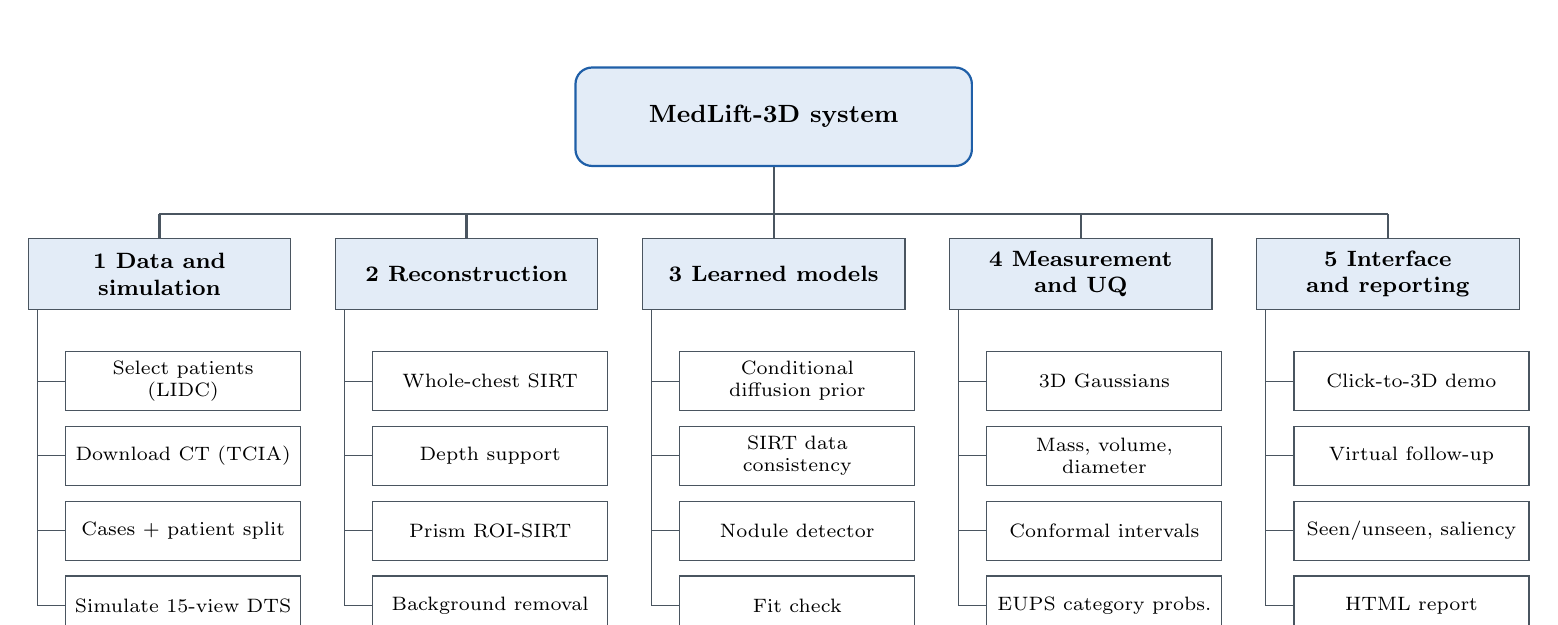
\begin{tikzpicture}[sub/.style={draw=edge, fill=accentlight, minimum width=3.3cm, minimum height=0.9cm, align=center, font=\footnotesize\bfseries, text width=3.1cm}]
  \node[mainproc, minimum width=5cm, text width=4.8cm, font=\small\bfseries] (root) at (7.8,2.0) {MedLift-3D system};
  \foreach \i/\n in {0/{1 Data and\\ simulation}, 1/{2 Reconstruction}, 2/{3 Learned models}, 3/{4 Measurement\\ and UQ}, 4/{5 Interface\\ and reporting}} {
    \node[sub] (s\i) at ({3.9*\i},0) {\n};
  }
  \draw[edge, thick] (root.south) -- ++(0,-0.6) coordinate (bus);
  \draw[edge, thick] (s0.north |- bus) -- (s4.north |- bus);
  \foreach \i in {0,...,4} { \draw[edge, thick] (s\i.north |- bus) -- (s\i.north); }
  \newcommand{\leaves}[5]{%
    \foreach \t [count=\k] in {{#2},{#3},{#4},{#5}} {
      \node[leaf] (l#1\k) at ($(s#1.south)+(0.3,{-0.95*\k+0.05})$) {\t};
      \draw[edge] ($(s#1.south west)+(0.12,0)$) |- (l#1\k.west);
    }}
  \leaves{0}{Select patients (LIDC)}{Download CT (TCIA)}{Cases + patient split}{Simulate 15-view DTS}
  \leaves{1}{Whole-chest SIRT}{Depth support}{Prism ROI-SIRT}{Background removal}
  \leaves{2}{Conditional diffusion prior}{SIRT data consistency}{Nodule detector}{Fit check}
  \leaves{3}{3D Gaussians}{Mass, volume, diameter}{Conformal intervals}{EUPS category probs.}
  \leaves{4}{Click-to-3D demo}{Virtual follow-up}{Seen/unseen, saliency}{HTML report}
\end{tikzpicture}
}
  \caption{Functional decomposition diagram: five subsystems and their functions.}
  \label{fig:fdd}
\end{figure}

\subsection{Entity-Relationship Model and Data Dictionary}

\Cref{fig:er} shows the data entities and their relationships: a patient has CT cases, a case contains nodules marked by three or four readers, and each nodule is measured by several methods, each measurement aggregating eight hypotheses that are fitted by Gaussian sets and calibrated per method. \Cref{tab:dict} gives the data dictionary.

\begin{figure}[htbp]
  \centering
  \resizebox{\linewidth}{!}{% Entity-relationship model (crow's-foot style cardinalities as labels)
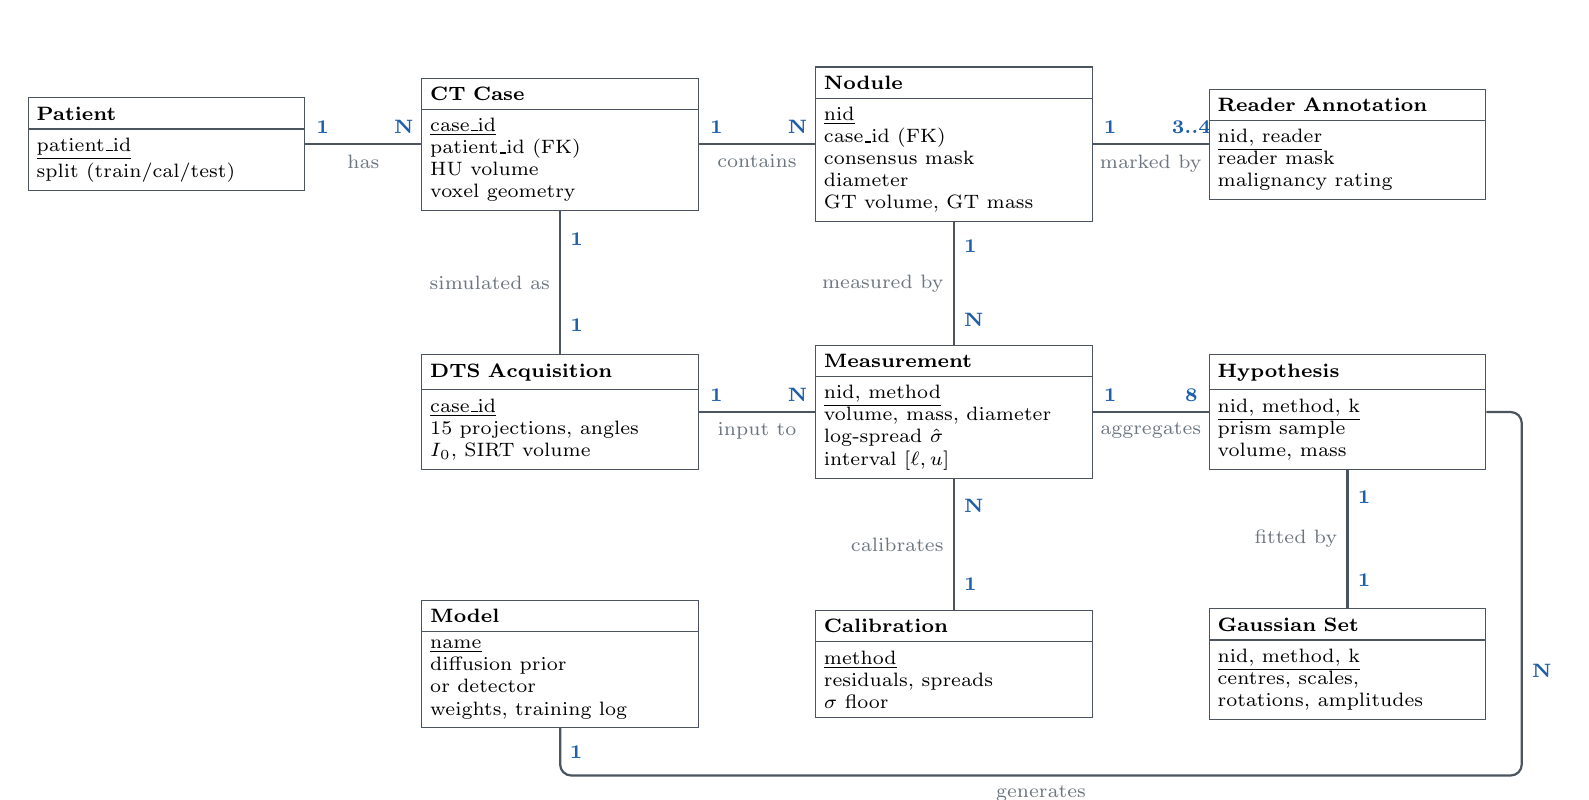
\begin{tikzpicture}[font=\scriptsize,
    ent/.style={draw=edge, fill=white, rectangle split, rectangle split parts=2, rectangle split part fill={accentlight,white},
                align=left, text width=3.3cm, inner sep=3pt},
    rel/.style={edge, thick},
    card/.style={font=\scriptsize\bfseries, text=accent}]
  \node[ent] (pat) at (0,0) {\textbf{Patient}\nodepart{second}\underline{patient\_id}\\ split (train/cal/test)};
  \node[ent] (case) at (5.0,0) {\textbf{CT Case}\nodepart{second}\underline{case\_id}\\ patient\_id (FK)\\ HU volume\\ voxel geometry};
  \node[ent] (nod) at (10.0,0) {\textbf{Nodule}\nodepart{second}\underline{nid}\\ case\_id (FK)\\ consensus mask\\ diameter\\ GT volume, GT mass};
  \node[ent] (rdr) at (15.0,0) {\textbf{Reader Annotation}\nodepart{second}\underline{nid, reader}\\ reader mask\\ malignancy rating};
  \node[ent] (dts) at (5.0,-3.4) {\textbf{DTS Acquisition}\nodepart{second}\underline{case\_id}\\ 15 projections, angles\\ $I_0$, SIRT volume};
  \node[ent] (meas) at (10.0,-3.4) {\textbf{Measurement}\nodepart{second}\underline{nid, method}\\ volume, mass, diameter\\ log-spread $\hat\sigma$\\ interval $[\ell,u]$};
  \node[ent] (hyp) at (15.0,-3.4) {\textbf{Hypothesis}\nodepart{second}\underline{nid, method, k}\\ prism sample\\ volume, mass};
  \node[ent] (gau) at (15.0,-6.6) {\textbf{Gaussian Set}\nodepart{second}\underline{nid, method, k}\\ centres, scales,\\ rotations, amplitudes};
  \node[ent] (cal) at (10.0,-6.6) {\textbf{Calibration}\nodepart{second}\underline{method}\\ residuals, spreads\\ $\sigma$ floor};
  \node[ent] (mdl) at (5.0,-6.6) {\textbf{Model}\nodepart{second}\underline{name}\\ diffusion prior\\ or detector\\ weights, training log};

  \draw[rel] (pat) -- node[card, above, pos=0.15] {1} node[card, above, pos=0.85] {N} node[below, text=quiet] {has} (case);
  \draw[rel] (case) -- node[card, above, pos=0.15] {1} node[card, above, pos=0.85] {N} node[below, text=quiet] {contains} (nod);
  \draw[rel] (nod) -- node[card, above, pos=0.15] {1} node[card, above, pos=0.85] {3..4} node[below, text=quiet] {marked by} (rdr);
  \draw[rel] (case) -- node[card, right, pos=0.2] {1} node[card, right, pos=0.8] {1} node[left, text=quiet] {simulated as} (dts);
  \draw[rel] (nod) -- node[card, right, pos=0.2] {1} node[card, right, pos=0.8] {N} node[left, text=quiet] {measured by} (meas);
  \draw[rel] (meas) -- node[card, above, pos=0.15] {1} node[card, above, pos=0.85] {8} node[below, text=quiet] {aggregates} (hyp);
  \draw[rel] (hyp) -- node[card, right, pos=0.2] {1} node[card, right, pos=0.8] {1} node[left, text=quiet] {fitted by} (gau);
  \draw[rel] (cal) -- node[card, right, pos=0.2] {1} node[card, right, pos=0.8] {N} node[left, text=quiet] {calibrates} (meas);
  \draw[rel, rounded corners=4pt] (mdl.south) -- ++(0,-0.6) -| node[card, right, pos=0.97] {N} node[below, pos=0.25, text=quiet] {generates} ($(gau.east)+(0.45,0)$) |- (hyp.east);
  \node[card, right] at ($(mdl.south)+(0,-0.3)$) {1};
  \draw[rel] (dts) -- node[card, above, pos=0.15] {1} node[card, above, pos=0.85] {N} node[below, text=quiet] {input to} (meas);
\end{tikzpicture}
}
  \caption{Entity-relationship model of MedLift-3D (keys underlined, cardinalities in blue).}
  \label{fig:er}
\end{figure}

\begin{table}[!htbp]
\centering\small
\caption{Data dictionary.}
\label{tab:dict}
\begin{tabularx}{\linewidth}{>{\raggedright\arraybackslash}p{3.1cm} >{\raggedright\arraybackslash}p{3.0cm} >{\raggedright\arraybackslash}X >{\raggedright\arraybackslash}p{2.8cm}}
\toprule
Store / item & Format & Contents & Constraint \\
\midrule
D1 Case & int16 + packed bits + JSON header & CT in HU, consensus and four reader masks per nodule, voxel geometry, patient ID & HU in $[-1024, 3071]$ \\
Projections & float, $15{\times}536{\times}536$ & Noisy line integrals per view & Finite, max $<15$ \\
D2 SIRT volume & float, 2.5~mm voxels & Whole-chest DTS reconstruction & Patient depth + 5~mm \\
Prism & float, $64{\times}128{\times}64$, $1{\times}2{\times}1$~mm & Column through the chest at the click & Rays $\geq$50\% inside \\
Training pair & float16 & Condition (DTS prism) and target (CT prism) in HU & Train patients only \\
D3 Diffusion model & PyTorch checkpoint & 17.42~M parameters, EMA weights & Selected on held-out train pairs \\
D3 Detector & PyTorch checkpoint & 0.34~M parameters, heatmap 3D U-Net & Selected on cal.\ patients \\
Gaussians & float32 & Centres ($N{\times}3$), scales ($N{\times}3$), quaternions ($N{\times}4$), amplitudes ($N$) & $N \leq \num{30000}$ \\
Result row & JSON lines & Per nodule and method: volume, mass, log-spread, members, ground truth & One row per nodule \\
D4 Calibration & JSON & Per method: residuals, spreads, $\sigma$ floor & Cal.\ patients only \\
Report & JSON / UI & Mass and volume with intervals, category probabilities, diameter, low-confidence flag, run time & Interval type stated \\
\bottomrule
\end{tabularx}
\end{table}

\subsection{What DTS Can Measure}

Let $f(x,y,z)$ be the nodule's excess attenuation, with $y$ the depth axis, and let the view at tube angle $\theta$ project along a direction tilted by $\theta$ from $y$ in the $y$--$z$ plane, with detector coordinates $(x, v)$ and $v$ along $\mathbf{e}_\theta = (0, -\sin\theta, \cos\theta)$. The moments of the projection $p_\theta$ are
\begin{align}
  \iint p_\theta(x,v)\,\mathrm{d}x\,\mathrm{d}v &= M, \label{eq:m0}\\
  \iint v\, p_\theta(x,v)\,\mathrm{d}x\,\mathrm{d}v &= -\sin\theta\, M y_c + \cos\theta\, M z_c, \label{eq:m1}\\
  \iint (v-\bar v)^2 p_\theta\,\mathrm{d}x\,\mathrm{d}v &= \sin^2\theta\, S_{yy} - 2\sin\theta\cos\theta\, S_{yz} + \cos^2\theta\, S_{zz}, \label{eq:m2}
\end{align}
where $M$ is the mass, $(y_c,z_c)$ the centroid and $S$ the second central moments (for a cone beam, \cref{eq:m0} holds up to a known magnification factor). Every view gives the mass directly (\cref{eq:m0}). The depth position enters only through $\sin\theta \leq \sin 15^\circ$, making it $1/\sin15^\circ \approx 3.9$ times worse conditioned than in-plane position, and the depth extent $S_{yy}$, which volume needs, enters through $\sin^2\theta$, about $1/\sin^2 15^\circ \approx 15$ times worse. Step~01 confirms this numerically: the detector integral matched the mass to 0.03\% in all 15 views, and an object three times deeper with equal mass gave the same integrals.

\subsection{Proposed Architecture}

\Cref{fig:pipeline} gives an overview of the method; its stages are described below.

\begin{figure}[htbp]
  \centering
  \resizebox{\linewidth}{!}{% MedLift-3D method overview (research-style pipeline figure)
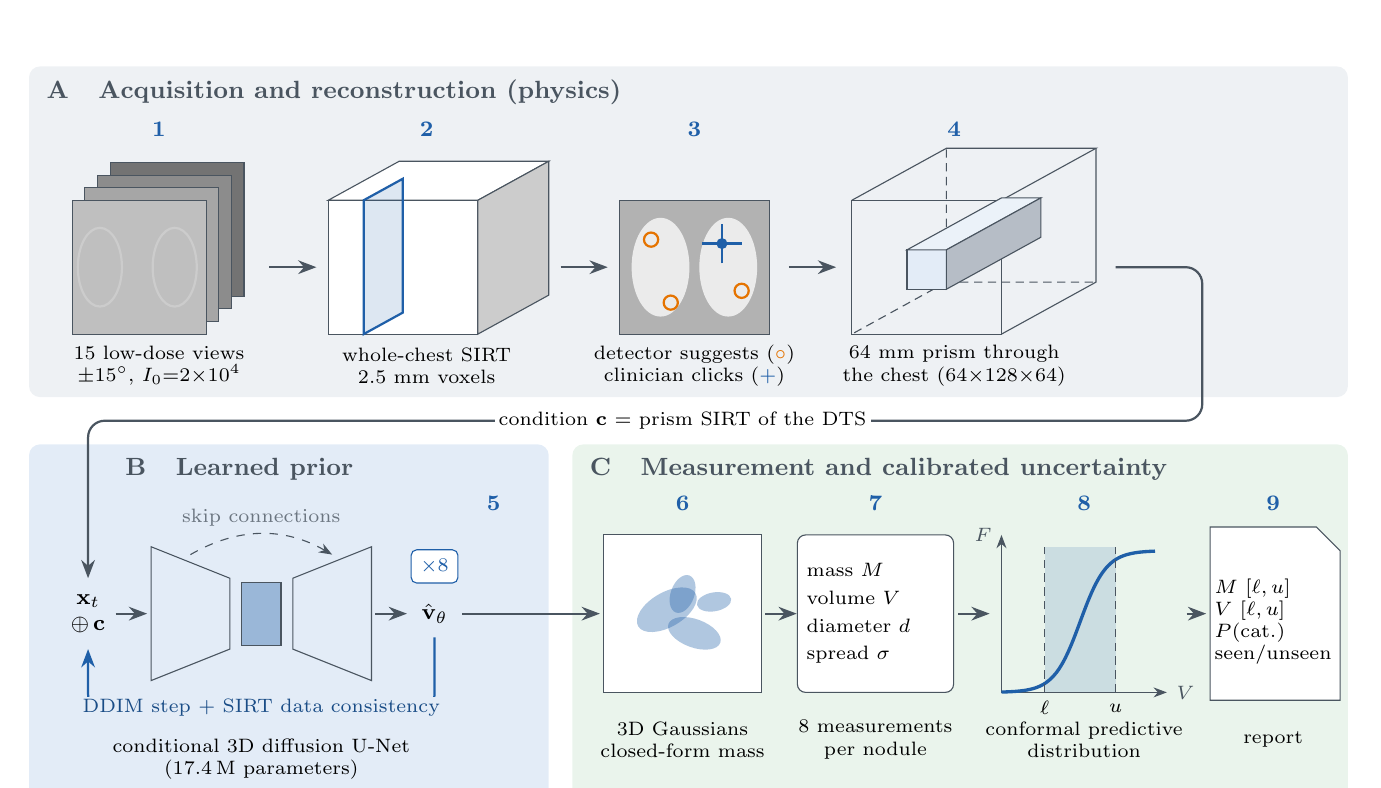
\begin{tikzpicture}[font=\footnotesize, >=Stealth,
    arr/.style={->, thick, edge},
    lbl/.style={align=center, font=\scriptsize, text width=3.1cm},
    stage/.style={font=\footnotesize\bfseries, text=accent},
    grp/.style={draw=edge!50, dashed, rounded corners=4pt, inner sep=6pt}]

  % cuboid: \cub{x}{y}{w}{h}{d}{fill}
  \newcommand{\cub}[6]{%
    \draw[edge, fill=#6] (#1,#2) rectangle ++(#3,#4);
    \draw[edge, fill=#6!70!white] (#1,#2+#4) -- ++(#5,0.55*#5) -- ++(#3,0) -- ++(-#5,-0.55*#5) -- cycle;
    \draw[edge, fill=#6!80!black] (#1+#3,#2) -- ++(#5,0.55*#5) -- ++(0,#4) -- ++(-#5,-0.55*#5) -- cycle;}

  % =================== row 1: acquisition and reconstruction (physics)
  \begin{scope}[on background layer]
    \fill[physics, rounded corners=4pt] (-0.3,4.35) rectangle (16.45,8.55);
  \end{scope}
  \node[anchor=north west, font=\small\bfseries, text=edge] at (-0.2,8.5) {A\quad Acquisition and reconstruction (physics)};

  % (1) projections: stack of views
  \foreach \i/\g in {3/55,2/45,1/35,0/25} {
    \draw[edge, fill=black!\g] ({0.25+0.16*\i},{5.15+0.16*\i}) rectangle ++(1.7,1.7);
  }
  \draw[white!80!black, thick] (0.6,6.0) ellipse (0.28 and 0.5);
  \draw[white!80!black, thick] (1.55,6.0) ellipse (0.28 and 0.5);
  \node[stage] at (1.35,7.75) {1};
  \node[lbl] at (1.35,4.75) {15 low-dose views\\ $\pm15^\circ$, $I_0{=}2{\times}10^4$};

  \draw[arr] (2.75,6.0) -- (3.35,6.0);

  % (2) whole-chest SIRT volume
  \cub{3.5}{5.15}{1.9}{1.7}{0.9}{white}
  \draw[accent, thick, fill=accent, fill opacity=0.15] (3.95,5.15) -- ++(0.9*0.55,0.55*0.9*0.55) -- ++(0,1.7) -- ++(-0.9*0.55,-0.55*0.9*0.55) -- cycle;
  \node[stage] at (4.75,7.75) {2};
  \node[lbl] at (4.75,4.75) {whole-chest SIRT\\ 2.5 mm voxels};

  \draw[arr] (6.45,6.0) -- (7.05,6.0);

  % (3) coronal slice + detector suggestions + click
  \draw[edge, fill=black!30] (7.2,5.15) rectangle ++(1.9,1.7);
  \draw[black!8, fill=black!8] (7.72,6.0) ellipse (0.36 and 0.62);
  \draw[black!8, fill=black!8] (8.58,6.0) ellipse (0.36 and 0.62);
  \foreach \p in {(7.6,6.35),(8.75,5.7),(7.85,5.55)} { \draw[orange!90!black, thick] \p circle (0.09); }
  \fill[accent] (8.5,6.3) circle (0.07);
  \draw[accent, thick] (8.5,6.05) -- ++(0,0.5) (8.25,6.3) -- ++(0.5,0);
  \node[stage] at (8.15,7.75) {3};
  \node[lbl] at (8.15,4.75) {detector suggests (\textcolor{orange!90!black}{$\circ$})\\ clinician clicks (\textcolor{accent}{$+$})};

  \draw[arr] (9.35,6.0) -- (9.95,6.0);

  % (4) prism through the chest
  \draw[edge] (10.15,5.15) rectangle ++(1.9,1.7);
  \draw[edge] (10.15,6.85) -- ++(1.2,0.66) -- ++(1.9,0) -- (12.05,6.85);
  \draw[edge] (13.25,7.51) -- ++(0,-1.7) -- (12.05,5.15);
  \draw[edge, densely dashed] (11.35,5.81) -- ++(1.9,0) (11.35,5.81) -- ++(0,1.7) (11.35,5.81) -- (10.15,5.15);
  \cub{10.85}{5.72}{0.5}{0.5}{1.2}{accentlight}
  \node[stage] at (11.45,7.75) {4};
  \node[lbl] at (11.45,4.75) {64 mm prism through\\ the chest ($64{\times}128{\times}64$)};

  % rows link
  \draw[arr, rounded corners=6pt] (13.5,6.0) -- (14.6,6.0) -- (14.6,4.05) -- (0.45,4.05) -- (0.45,2.05);
  \node[font=\scriptsize, fill=white, inner sep=1.5pt] at (8.0,4.05) {condition $\mathbf{c}$ = prism SIRT of the DTS};

  % =================== row 2: learned prior | measurement and uncertainty
  \begin{scope}[on background layer]
    \fill[learned, rounded corners=4pt] (-0.3,-0.75) rectangle (6.3,3.75);
    \fill[measure, rounded corners=4pt] (6.6,-0.75) rectangle (16.45,3.75);
  \end{scope}
  \node[anchor=north west, font=\small\bfseries, text=edge] at (0.8,3.7) {B\quad Learned prior};
  \node[anchor=north west, font=\small\bfseries, text=edge] at (6.7,3.7) {C\quad Measurement and calibrated uncertainty};

  % (5) conditional 3D U-Net
  \draw[edge, fill=accentlight] (1.25,0.75) -- (2.25,1.15) -- (2.25,2.05) -- (1.25,2.45) -- cycle;
  \draw[edge, fill=accent!45] (2.4,1.2) rectangle (2.9,2.0);
  \draw[edge, fill=accentlight] (3.05,1.15) -- (4.05,0.75) -- (4.05,2.45) -- (3.05,2.05) -- cycle;
  \draw[edge, dashed, ->] (1.75,2.35) to[bend left=30] (3.55,2.35);
  \node[font=\scriptsize, text=quiet] at (2.65,2.82) {skip connections};
  \node[align=center] at (0.45,1.6) {$\mathbf{x}_t$\\ $\oplus\,\mathbf{c}$};
  \draw[arr] (0.8,1.6) -- (1.2,1.6);
  \draw[arr] (4.1,1.6) -- (4.5,1.6);
  \node at (4.85,1.6) {$\hat{\mathbf{v}}_\theta$};
  \node[draw=accent, fill=white, rounded corners=2pt, font=\scriptsize\bfseries, text=accent] at (4.85,2.2) {$\times 8$};
  \draw[arr, accent, rounded corners=5pt] (4.85,1.3) -- (4.85,0.4) -- (0.45,0.4) -- (0.45,1.15);
  \node[font=\scriptsize, fill=learned, inner sep=1pt, text=accent!80!black] at (2.65,0.4) {DDIM step + SIRT data consistency};
  \node[stage] at (5.6,3.0) {5};
  \node[lbl, text width=5cm] at (2.65,-0.25) {conditional 3D diffusion U-Net\\ (17.4\,M parameters)};

  \draw[arr] (5.2,1.6) -- (6.95,1.6);

  % (6) 3D Gaussians
  \draw[edge, fill=white] (7.0,0.6) rectangle ++(2.0,2.0);
  \foreach \cx/\cy/\rx/\ry/\r in {7.8/1.65/0.42/0.22/30, 8.15/1.35/0.35/0.18/-20, 8.0/1.85/0.25/0.15/70, 8.4/1.75/0.22/0.12/10} {
    \fill[accent, opacity=0.35, rotate around={\r:(\cx,\cy)}] (\cx,\cy) ellipse (\rx cm and \ry cm);
  }
  \node[stage] at (8.0,3.0) {6};
  \node[lbl, text width=2.4cm] at (8.0,0.0) {3D Gaussians\\ closed-form mass};

  \draw[arr] (9.05,1.6) -- (9.45,1.6);

  % (7) measurements
  \node[draw=edge, fill=white, rounded corners=3pt, align=left, text width=1.75cm, minimum height=2.0cm, font=\scriptsize] at (10.45,1.6)
    {mass $M$\\[2pt] volume $V$\\[2pt] diameter $d$\\[2pt] spread $\sigma$};
  \node[stage] at (10.45,3.0) {7};
  \node[lbl, text width=2.2cm] at (10.45,0.0) {8 measurements\\ per nodule};

  \draw[arr] (11.5,1.6) -- (11.9,1.6);

  % (8) conformal predictive distribution
  \begin{scope}[shift={(12.05,0.6)}]
    \draw[->, edge] (0,0) -- (2.1,0) node[right, font=\scriptsize] {$V$};
    \draw[->, edge] (0,0) -- (0,2.0) node[left, font=\scriptsize] {$F$};
    \fill[accent, opacity=0.15] (0.55,0) rectangle (1.45,1.85);
    \draw[accent, very thick, domain=0:1.95, samples=60, smooth] plot (\x, {1.8/(1+exp(-6*(\x-1.0)))});
    \draw[edge, densely dashed] (0.55,0) -- (0.55,1.85) (1.45,0) -- (1.45,1.85);
    \node[font=\scriptsize] at (0.55,-0.2) {$\ell$};
    \node[font=\scriptsize] at (1.45,-0.2) {$u$};
  \end{scope}
  \node[stage] at (13.1,3.0) {8};
  \node[lbl, text width=3.2cm] at (13.1,0.0) {conformal predictive\\ distribution};

  \draw[arr] (14.4,1.6) -- (14.65,1.6);

  % (9) report
  \draw[edge, fill=white] (14.7,0.5) -- ++(1.65,0) -- ++(0,1.9) -- ++(-0.3,0.3) -- ++(-1.35,0) -- cycle;
  \node[align=left, font=\scriptsize] at (15.5,1.5) {$M\ [\ell,u]$\\ $V\ [\ell,u]$\\ $P(\mathrm{cat.})$\\ seen/unseen};
  \node[stage] at (15.5,3.0) {9};
  \node[lbl, text width=1.8cm] at (15.5,0.0) {report};
\end{tikzpicture}
}
  \caption[MedLift-3D method overview]{MedLift-3D method overview. (A) Physics: low-dose DTS is simulated, reconstructed and cut to a prism around the click. (B) A conditional 3D diffusion prior generates eight hypotheses of the prism, each kept consistent with the X-rays. (C) Gaussians give closed-form mass; the eight measurements are calibrated into intervals and category probabilities.}
  \label{fig:pipeline}
\end{figure}

\paragraph{Stage 1: simulated low-dose DTS.} The CT table is removed, then 15 views over $\pm15^\circ$ are simulated at CT resolution with 0.5~mm ray sampling, SID 1800~mm, a 43~cm flat panel with 0.8~mm pixels, monochromatic attenuation and Poisson noise at $I_0 = 2\times10^4$. The geometry matches the GE VolumeRAD sweep; reconstruction uses different grids than simulation to avoid the inverse crime.

\paragraph{Stage 2: whole-chest SIRT with depth support.} SIRT (40 iterations, 2.5~mm voxels) is confined in depth to the patient (body outline + 5~mm). Without this support the reconstruction placed attenuation in the air in front of and behind the patient, and on real chests the prism lost about a third of its attenuation; with it the prism keeps 98.7\%.

\paragraph{Stage 3: learned detector.} A small 3D U-Net~\cite{cicek2016unet} (0.34~M parameters) predicts a nodule heatmap from the SIRT volume, and its peaks are offered as suggestions. A Laplacian-of-Gaussian and Hessian blob detector is the training-free baseline.

\paragraph{Stage 4: prism ROI.} Around the click, a $64\times64$~mm column through the whole chest ($64\times128\times64$ voxels at $1\times2\times1$~mm) is reconstructed by SIRT using only rays that carry at least 50\% of their attenuation inside the prism; the rest of the chest is subtracted using the coarse reconstruction. Depth is kept whole because each ray's attenuation is spread along its full path: a small 3D box around the nodule gave a 73\% error against 5--7\% for the prism.

\paragraph{Stage 5: conditional 3D diffusion prior.} A 3D U-Net (\cref{fig:unet}; base 32 channels, multipliers 1/2/4/4, two residual blocks per level, attention at the lowest level, 17.42~M parameters) learns $p(\text{CT prism}\mid\text{DTS prism})$ with v-prediction, a cosine schedule over 1000 steps, EMA weights and bf16 mixed precision. Sampling uses 50 DDIM steps; from 60\% of the way through, every denoised estimate $\hat{\mathbf{x}}_0$ receives two SIRT data-consistency iterations,
\begin{equation}
  \hat{\mathbf{x}}_0 \leftarrow \hat{\mathbf{x}}_0 + \lambda\, C A^{\top} R\,(\mathbf{b} - A\hat{\mathbf{x}}_0),
\end{equation}
before the next DDIM step. Eight samples give eight hypotheses that agree with the X-rays but differ where the X-rays are blind.



\paragraph{Stage 6: 3D Gaussians and measurement.} For each hypothesis the nodule box ($40\times50\times40$~mm) is fitted with anisotropic Gaussians (100 fitting and 100 refinement iterations against the measured projections, the rest of the prism fixed). A seeded half-maximum segmentation, confined to a plausible nodule extent, gives the volume; \cref{eq:gaussmass} gives the mass; and the long-axis 2D diameter is kept as the clinical baseline.

\paragraph{Stage 7: uncertainty.} The eight hypotheses give a log-scale spread $\hat\sigma$. On the calibration patients this spread is calibrated with (a) split-conformal asymmetric intervals (step~10) and (b) normalised and Mondrian conformal predictive systems with crepes (step~16), which give full predictive distributions, EUPS category probabilities and category sets.

\paragraph{Stage 8: growth.} Each nodule is grown in the CT by a known factor, its projections are updated and fresh noise added; VDT and MDT are measured and assigned to the NELSON categories.

\paragraph{Stage 9: explanation.} The true CT prism is split into seen and unseen parts by conjugate-gradient least squares (CGLS)~\cite{hestenes1952cg} on the prism projection operator. We measure how much of the nodule's mass and shape lies in each part and the prior's \emph{unseen skill}, the correlation of its unseen content with the truth's (\cref{fig:seen}). Input$\times$gradient saliency explains the detector, and rank correlations relate the measurement error to nodule size, depth and contrast.

\subsection{Diffusion Network Architecture}

\Cref{fig:unet} shows the conditional 3D U-Net. The noisy prism and the DTS condition enter as two channels; four resolution levels with 32, 64, 128 and 128 channels use two residual blocks each in the encoder and three in the decoder, with skip connections between them; multi-head self-attention runs at the coarsest level ($8{\times}16{\times}8$) and in the bottleneck; and a sinusoidal timestep embedding passed through an MLP is added inside every residual block. The output layer is initialised to zero so that training starts from a stable state.

\begin{figure}[htbp]
  \centering
  \resizebox{0.95\linewidth}{!}{% Conditional 3D U-Net of the diffusion prior (medlift3d/diffusion/unet3d.py)
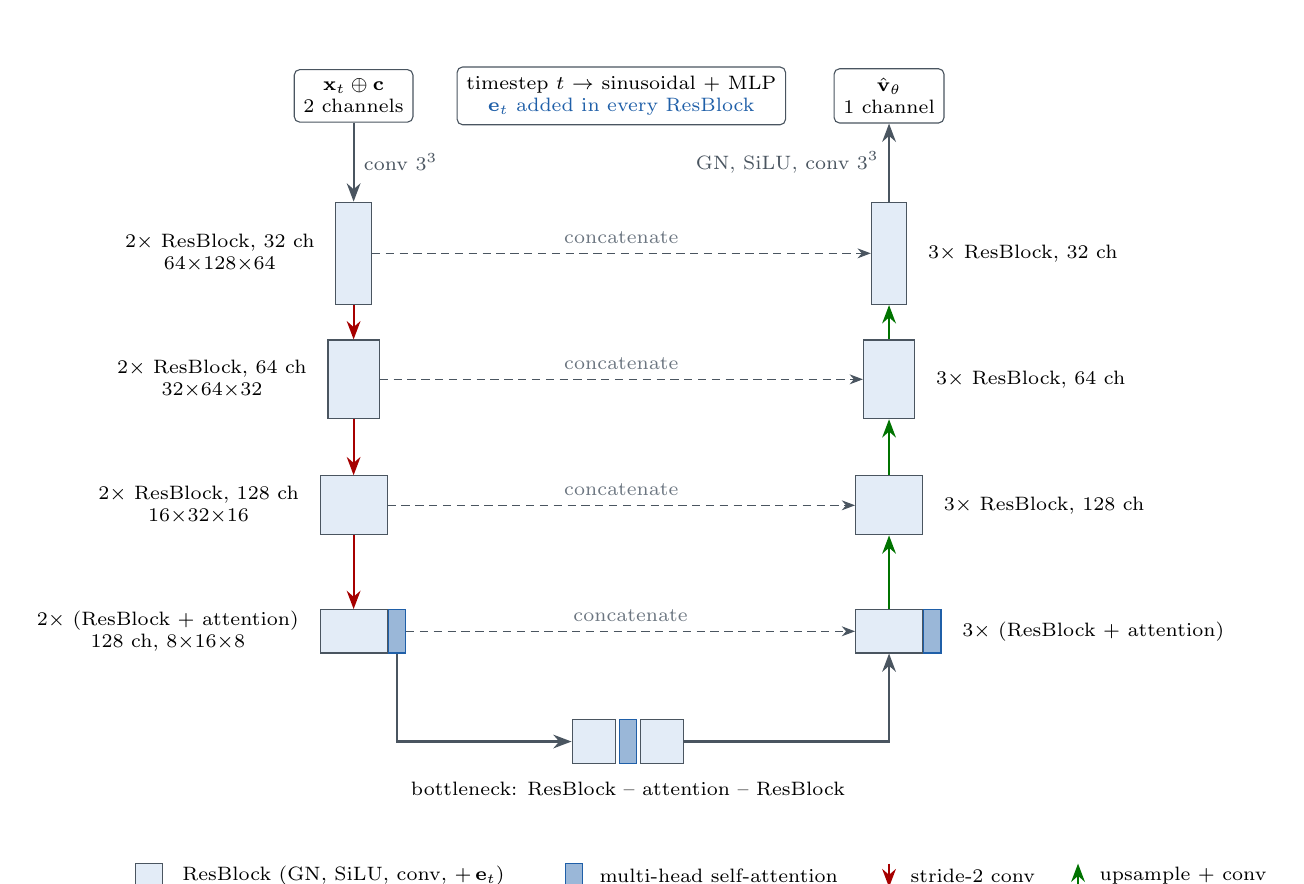
\begin{tikzpicture}[font=\footnotesize, >=Stealth,
    res/.style={draw=edge, fill=accentlight, minimum width=#1, inner sep=0pt},
    att/.style={draw=accent, fill=accent!45, minimum width=0.22cm, inner sep=0pt},
    down/.style={->, thick, red!65!black},
    up/.style={->, thick, green!45!black},
    skip/.style={->, densely dashed, edge},
    lab/.style={font=\scriptsize, align=center}]

  % level geometry: y centre, block height (resolution), block width (channels)
  \def\yA{6.0}\def\yB{4.4}\def\yC{2.8}\def\yD{1.2}
  \def\xe{3.2}\def\xd{10.0}

  % ----- encoder
  \node[res=0.45cm, minimum height=1.3cm] (e0) at (\xe,\yA) {};
  \node[res=0.65cm, minimum height=1.0cm] (e1) at (\xe,\yB) {};
  \node[res=0.85cm, minimum height=0.75cm] (e2) at (\xe,\yC) {};
  \node[res=0.85cm, minimum height=0.55cm] (e3) at (\xe,\yD) {};
  \node[att, minimum height=0.55cm, right=0pt of e3] (a3) {};
  \node[lab, left=4pt of e0] {$2\times$ ResBlock, 32 ch\\ $64{\times}128{\times}64$};
  \node[lab, left=4pt of e1] {$2\times$ ResBlock, 64 ch\\ $32{\times}64{\times}32$};
  \node[lab, left=4pt of e2] {$2\times$ ResBlock, 128 ch\\ $16{\times}32{\times}16$};
  \node[lab, left=4pt of e3] {$2\times$ (ResBlock + attention)\\ 128 ch, $8{\times}16{\times}8$};
  \draw[down] (e0.south) -- (e1.north);
  \draw[down] (e1.south) -- (e2.north);
  \draw[down] (e2.south) -- (e3.north);

  % ----- bottleneck
  \node[res=0.55cm, minimum height=0.55cm] (m1) at (6.25,-0.2) {};
  \node[att, minimum height=0.55cm, right=1pt of m1] (ma) {};
  \node[res=0.55cm, minimum height=0.55cm, right=1pt of ma] (m2) {};
  \node[lab, below=3pt of ma] {bottleneck: ResBlock -- attention -- ResBlock};
  \draw[->, thick, edge] (a3.south) |- (m1.west);

  % ----- decoder
  \node[res=0.85cm, minimum height=0.55cm] (d3) at (\xd,\yD) {};
  \node[att, minimum height=0.55cm, right=0pt of d3] (b3) {};
  \node[res=0.85cm, minimum height=0.75cm] (d2) at (\xd,\yC) {};
  \node[res=0.65cm, minimum height=1.0cm] (d1) at (\xd,\yB) {};
  \node[res=0.45cm, minimum height=1.3cm] (d0) at (\xd,\yA) {};
  \draw[->, thick, edge] (m2.east) -| (d3.south);
  \draw[up] (d3.north) -- (d2.south);
  \draw[up] (d2.north) -- (d1.south);
  \draw[up] (d1.north) -- (d0.south);
  \node[lab, right=4pt of b3] {$3\times$ (ResBlock + attention)};
  \node[lab, right=4pt of d2] {$3\times$ ResBlock, 128 ch};
  \node[lab, right=4pt of d1] {$3\times$ ResBlock, 64 ch};
  \node[lab, right=4pt of d0] {$3\times$ ResBlock, 32 ch};

  % ----- skips
  \foreach \e/\d in {e0/d0, e1/d1, e2/d2} { \draw[skip] (\e.east) -- node[above, lab, text=quiet]{concatenate} (\d.west); }
  \draw[skip] (a3.east) -- node[above, lab, text=quiet]{concatenate} (d3.west);

  % ----- input / output
  \node[draw=edge, fill=white, rounded corners=2pt, lab] (in) at (\xe,8.0) {$\mathbf{x}_t \oplus \mathbf{c}$\\ 2 channels};
  \draw[->, thick, edge] (in.south) -- node[right, lab]{conv $3^3$} (e0.north);
  \node[draw=edge, fill=white, rounded corners=2pt, lab] (out) at (\xd,8.0) {$\hat{\mathbf{v}}_\theta$\\ 1 channel};
  \draw[->, thick, edge] (d0.north) -- node[left, lab]{GN, SiLU, conv $3^3$} (out.south);

  % ----- time embedding
  \node[draw=edge, fill=white, rounded corners=2pt, lab] (t) at (6.6,8.0) {timestep $t$ $\rightarrow$ sinusoidal + MLP\\ \textcolor{accent}{$\mathbf{e}_t$ added in every ResBlock}};

  % ----- legend
  \begin{scope}[shift={(0.6,-1.9)}]
    \node[res=0.35cm, minimum height=0.3cm] at (0,0) {}; \node[lab, anchor=west] at (0.3,0) {ResBlock (GN, SiLU, conv, $+\,\mathbf{e}_t$)};
    \node[att, minimum height=0.3cm] at (5.4,0) {}; \node[lab, anchor=west] at (5.6,0) {multi-head self-attention};
    \draw[down] (9.4,0.15) -- (9.4,-0.15); \node[lab, anchor=west] at (9.55,0) {stride-2 conv};
    \draw[up] (11.8,-0.15) -- (11.8,0.15); \node[lab, anchor=west] at (11.95,0) {upsample + conv};
  \end{scope}
\end{tikzpicture}
}
  \caption[Conditional 3D U-Net of the diffusion prior]{Conditional 3D U-Net of the diffusion prior. The noisy prism $\mathbf{x}_t$ is concatenated with the DTS condition $\mathbf{c}$; the timestep embedding is added in every residual block; the network predicts the velocity $\hat{\mathbf{v}}_\theta$.}
  \label{fig:unet}
\end{figure}

\subsection{Alternative Solutions}

 \Cref{tab:alternatives} lists the alternatives and why they were rejected. The initial design of this project generated whole $512^3$ volumes with a latent diffusion model; it is included in the table because its lessons shaped the final design: a large generator judged by training losses could not show whether a single nodule measurement was right, so the goal was narrowed to clinical numbers that can be verified.

\begin{table}[!htbp]
\centering\small
\caption{Alternative solutions and the rationale for the selected design.}
\label{tab:alternatives}
\begin{tabularx}{\linewidth}{>{\raggedright\arraybackslash}p{3.4cm} >{\raggedright\arraybackslash}X >{\raggedright\arraybackslash}p{3.6cm}}
\toprule
Alternative & Why rejected & Selected instead \\
\midrule
FBP or SIRT alone & Cannot fill the missing wedge; physics-only volume errors of 80--90\% on small nodules & SIRT as input and data-consistency step, plus a learned prior \\
Neural radiance fields~\cite{mildenhall2020nerf} & Slow per-patient optimisation, implicit geometry, no prior for unseen depth & Explicit 3D Gaussians with closed-form mass \\
Whole-volume latent diffusion at $512^3$ (initial design) & Too large to train and verify with our resources; evaluated by generative losses, not clinical numbers & Small conditional prior on a prism, judged by calibrated measurements \\
Small 3D box ROI & Each ray's attenuation lies mostly outside the box: 73\% error vs 5--7\% & Prism through the whole chest \\
GAN prior & Training instability; one output per input & Diffusion: stable training, many hypotheses \\
Unconditional prior with posterior sampling only & Slower and weaker for a strongly ill-posed \ang{30} problem & Conditional model + SIRT data consistency \\
Raw ensemble variance or MC dropout & Not calibrated; no coverage guarantee & Ensemble spread calibrated by conformal prediction \\
Volume-only reporting & Volume depends on the poorly measured depth & Mass first, volume second, both with intervals \\
\bottomrule
\end{tabularx}
\end{table}

\section{Project Plan}

MedLift-3D was developed over twelve months in an iterative research and development cycle, organised in four phases that match the task groups of the Gantt chart in \cref{fig:gantt}. The iterative approach suits the experimental nature of generative AI: the prior, the measurement and the uncertainty layer were revised whenever an intermediate verification step showed a problem.

\paragraph{Phase 1: Inception, data and feasibility (months 1--3).} \emph{Objective:} establish the theoretical basis and a reliable data pipeline. \emph{Tasks:} 1.1 literature review and ethics, 1.2 dataset acquisition and preprocessing, 1.3 DTS simulation, 1.4 baseline reconstruction. \emph{Deliverables:} literature review, curated LIDC-IDRI cases with consensus masks, the DTS simulator and baseline SIRT results.

\paragraph{Phase 2: Core generative architecture (months 3--6).} \emph{Objective:} build and train the learned prior. \emph{Tasks:} 2.1 projection physics and its verification (including the projection-moment analysis), 2.2 prism ROI reconstruction, 2.3 conditional diffusion prior with data consistency, 2.4 diffusion training. \emph{Deliverables:} verified differentiable projector, prism reconstruction, trained diffusion prior.

\paragraph{Phase 3: Gaussians, detection and uncertainty (months 6--9).} \emph{Objective:} turn reconstructions into calibrated, explainable measurements. \emph{Tasks:} 3.1 Gaussian parameterisation and closed-form mass, 3.2 nodule detector, 3.3 conformal uncertainty, 3.4 explainability. \emph{Deliverables:} measurement module, detector, calibrated intervals and probabilities, seen/unseen analysis.

\paragraph{Phase 4: Validation, interface and deployment (months 9--12).} \emph{Objective:} evaluate the complete system and deliver it. \emph{Tasks:} 4.1 pilot and full-scale evaluation, 4.2 growth and sensitivity studies, 4.3 user interface development, 4.4 documentation and defense. \emph{Deliverables:} results of the 583-patient study, the click-to-3D application, the final report.

\begin{sidewaysfigure}
  \centering
  \resizebox{0.95\textheight}{!}{% FYDP-III schedule (weeks of the trimester)
\begin{ganttchart}[
    hgrid, vgrid={*{8}{dotted}},
    x unit=1.15cm, y unit chart=0.52cm,
    title height=1, title label font=\footnotesize\bfseries,
    bar/.append style={fill=accentlight, draw=accent},
    bar label font=\footnotesize, bar height=0.55,
    group/.append style={fill=edge!70, draw=edge}, group label font=\footnotesize\bfseries,
    group peaks height=.2, group peaks tip position=0, group left shift=0, group right shift=0, group peaks width=0.2,
    milestone/.append style={fill=accent, draw=accent}, milestone left shift=-0.5, milestone right shift=-0.5, milestone label font=\footnotesize\itshape,
    link/.style={->, thick, edge}]{1}{9}
  \gantttitle{FYDP-III trimester (weeks)}{9} \\
  \gantttitlelist{1,...,9}{1} \\
  \ganttgroup{Analysis and design}{1}{3} \\
  \ganttbar{Problem re-analysis, projection moments}{1}{2} \\
  \ganttbar{Requirements, design, verification plan}{2}{3} \\
  \ganttgroup{Implementation}{2}{8} \\
  \ganttbar[name=phys]{Physics, DTS simulation, unit tests}{2}{4} \\
  \ganttbar[name=rec]{SIRT, prism ROI, 3D Gaussians}{3}{5} \\
  \ganttbar[name=dif]{Diffusion prior and training}{4}{6} \\
  \ganttbar{Detector, conformal UQ, growth}{5}{7} \\
  \ganttbar{Explainability, demo, HTML report}{6}{8} \\
  \ganttgroup{Verification and study}{6}{9} \\
  \ganttbar[name=pilot]{Real-data pilots (4 and 40 patients)}{6}{7} \\
  \ganttmilestone[name=full]{Full 583-patient run}{8} \\
  \ganttbar{Report, slides, defense}{8}{9} \\
  \ganttmilestone{Final submission}{9}
  \ganttlink{phys}{rec}
  \ganttlink{rec}{dif}
  \ganttlink{pilot}{full}
\end{ganttchart}
}
  \caption{Gantt chart of the twelve-month project schedule, by phase and task.}
  \label{fig:gantt}
\end{sidewaysfigure}

\section{Task Allocation}

Responsibilities were allocated according to the technical area in which each member is strongest, so that the critical paths of theoretical modelling, system optimisation and application engineering could progress in parallel. The mathematically intensive parts (the diffusion prior, its conditioning and data consistency, and the statistical calibration) need a solid theoretical grounding and were led by the lead AI architect. The systems engineer focused on performance and infrastructure, making the volumetric reconstruction feasible in GPU memory and running the computation on cloud GPUs. The full-stack developer connected the algorithms to clinical use, ensuring data quality, the user interface and the evaluation outputs. Every pipeline step has one owner who is accountable for its PASS/FAIL checks, and all members reviewed every step before the full run. \Cref{tab:tasks} gives the detailed allocation.

\begin{table}[!htbp]
\centering\small
\caption{Detailed task allocation matrix.}
\label{tab:tasks}
\begin{tabularx}{\linewidth}{>{\raggedright\arraybackslash}p{3.2cm} >{\raggedright\arraybackslash}p{3.0cm} >{\raggedright\arraybackslash}X}
\toprule
Team member & Role and focus & Detailed responsibilities \\
\midrule
Jubair Ahmed (011222136) & Lead AI architect (theoretical modelling) &
\textbullet~Projection-moment analysis of what DTS can measure \newline \textbullet~Design and mathematical formulation of the conditional diffusion prior (v-prediction, cosine schedule, DDIM sampling) \newline \textbullet~SIRT data-consistency sampling to suppress anatomical hallucination \newline \textbullet~Conformal intervals and calibrated category probabilities \\
\midrule
Foyez Ahammed Naeem (011222011) & Systems engineer (optimisation and backend) &
\textbullet~Differentiable DTS projector and memory-efficient prism reconstruction \newline \textbullet~GPU optimisation of training and sampling (mixed precision, batch sizing) \newline \textbullet~3D Gaussian fitting and closed-form mass; nodule detector training \newline \textbullet~Cloud infrastructure (RunPod CPU and GPU pods, Kaggle), the full run and backups \\
\midrule
Md Motasim Billah (011222016) & Full-stack developer (data and visualisation) &
\textbullet~Data curation and preprocessing of LIDC-IDRI (selection, consensus masks, DTS simulation inputs) \newline \textbullet~Clinician-facing click-to-3D interface with interactive 3D visualisation \newline \textbullet~Automated evaluation pipelines: accuracy, growth and explainability outputs, HTML report \\
\midrule
All members & -- & Literature review, verification of every PASS/FAIL step, report writing and presentation \\
\bottomrule
\end{tabularx}
\end{table}

\section{Summary}

The requirements were elicited from guidelines, the supervisor and published limits, negotiated where they conflicted, and specified with measurable acceptance criteria. The design measures mass first, reconstructs a prism around the click, fills depth with a data-consistent diffusion prior, measures with Gaussians, and calibrates and explains every number. \Cref{ch:results} verifies each requirement.

\chapter{Implementation and Results}
\label{ch:results}

This chapter describes the hardware and tools, how every requirement was verified, and the results for hypotheses H1--H6. All numbers come from the full run of October 27, 2026 on held-out test patients unless stated otherwise.

\section{Environment Setup}

\paragraph{Hardware.} \Cref{tab:hardware} lists the computing resources. CPU-only work (downloading about 64~GB of CT and building the cases) ran on a cheap CPU machine, and both machines shared one network volume so that the GPU machine started from the finished cases.

\begin{table}[htbp]
\centering\small
\caption{Computing resources.}
\label{tab:hardware}
\begin{tabularx}{\linewidth}{>{\raggedright\arraybackslash}p{3.3cm} >{\raggedright\arraybackslash}X >{\raggedright\arraybackslash}p{3.0cm} >{\raggedright\arraybackslash}p{1.8cm}}
\toprule
Resource & Used for & Specification & Cost \\
\midrule
Laptop / Kaggle CPU & Unit tests; synthetic-phantom smoke test & 4 cores & Free \\
Kaggle notebook & 40-patient pilot run; final demo and report viewer & $2\times$ NVIDIA T4, 16~GB & Free \\
RunPod CPU pod & Steps 02--04: patient selection, TCIA download, case building & Rented CPU & $<$ US\$2 \\
RunPod GPU pod & Steps 05--18: simulation, training, evaluation & NVIDIA L40S, 48~GB & about US\$1/h \\
RunPod network volume & Shared storage between pods; backup after every step & Persistent volume & included \\
\bottomrule
\end{tabularx}
\end{table}

\paragraph{Software and tools.} \Cref{tab:tools} lists the tools with the alternatives considered.

\begin{table}[htbp]
\centering\small
\caption{Software tools and the reasons for choosing them.}
\label{tab:tools}
\begin{tabularx}{\linewidth}{>{\raggedright\arraybackslash}p{3.3cm} >{\raggedright\arraybackslash}X >{\raggedright\arraybackslash}X}
\toprule
Tool & Role & Why chosen (alternative) \\
\midrule
Python 3.11+ & All code & Standard for medical AI (MATLAB: licence cost) \\
PyTorch 2.x & Projector, diffusion U-Net, detector, Gaussians; bf16 mixed precision & Differentiable physics and models in one framework \\
Own ray-driven projector (PyTorch) & DTS forward and back projection with gradients & Exact DTS geometry, differentiable, no CUDA build (ASTRA: separate build, no autograd) \\
pydicom, pylidc & LIDC DICOM and the four radiologists' annotations & Official annotation access \\
NumPy, SciPy, scikit-image & Morphology, segmentation, metrics & Mature and tested \\
crepes, scikit-learn & Conformal predictive systems; calibration metrics & Peer-reviewed implementation~\cite{bostrom2022crepes} \\
Gradio & Browser application & Quick UI in Python (Flask + JavaScript: more work) \\
Matplotlib, pytest & Figures; 69 unit tests & Standard \\
bash, tmux & Unattended 14-hour run with resume and backups & Survives disconnections \\
Git, GitHub & Version control & Team collaboration \\
\bottomrule
\end{tabularx}
\end{table}

\paragraph{Configuration and pipeline.} One YAML file holds every setting (geometry, dose, prism size, network size, sampling steps, number of hypotheses, $\alpha=0.1$) and the random seed is fixed. The pipeline has 18 scripted steps: 00 environment check, 01 physics verification, 02 patient selection, 03 TCIA download, 04 cases and split, 05 DTS simulation, 06 SIRT, 07 training pairs, 08 diffusion training, 09 per-nodule pipeline, 10 evaluation and conformal intervals, 11 growth, 12 demo, 13 geometry sensitivity, 14 detector, 15 fit check, 16 conformal predictive systems, 17 explainability and 18 HTML report. Each step prints PASS/FAIL lines with the expected value.

\section{Testing and Evaluation}

\paragraph{Verification strategy.} Testing was done at four levels:
\begin{enumerate}
  \item \textbf{Unit tests (69):} projector adjointness and mass conservation, the Gaussian mass formula, conformal coverage on synthetic data, Mondrian group coverage, CPS probabilities against crepes, the CGLS seen/unseen split, and fit-check parsing.
  \item \textbf{Smoke test:} the full pipeline on synthetic chest phantoms on a CPU in 10--20 minutes.
  \item \textbf{Real-data pilots:} 4 patients on CPU and 40 patients on Kaggle, which exposed and fixed the depth-support bug (prism attenuation 67--81\% $\rightarrow$ 98.7\%).
  \item \textbf{Full run:} 583 patients with automatic checks after every step and an HTML report listing all checks.
\end{enumerate}

\paragraph{Data split.} Patients, not nodules, were split 60/20/20: 350 training, 117 calibration and 116 test patients. The diffusion model was selected on 10\% of the training patients held out, the detector on the calibration patients, and the conformal methods were calibrated on the calibration patients. Test patients were used only for the final tables.

\paragraph{Metrics and baselines.} Volume and mass error (median signed error, median absolute percentage error MdAPE, Bland--Altman limits), failure rate, nodule-box PSNR, interval coverage and median width, Brier score and expected calibration error (ECE) of category probabilities, doubling-time error and NELSON category accuracy, detection CPM and sensitivity, seen fraction and unseen skill, and run time. Baselines: 2D diameter converted to a sphere volume (clinical practice), coarse SIRT, prism ROI-SIRT, physics-only Gaussians, and diffusion without Gaussians.

\paragraph{Requirement verification.} \Cref{tab:verify} traces every requirement of \cref{tab:fr,tab:nfr} to its measured result.

{\small
\begin{longtable}{>{\raggedright\arraybackslash}p{1.4cm} >{\raggedright\arraybackslash}p{4.3cm} >{\raggedright\arraybackslash}p{6.6cm} >{\raggedright\arraybackslash}p{1.3cm}}
\caption{Requirement verification (traceability).}\label{tab:verify}\\
\toprule
Req. & Criterion & Result & Met \\
\midrule
\endfirsthead
\toprule
Req. & Criterion & Result & Met \\
\midrule
\endhead
FR-01 & Positions agree; splits disjoint & DICOM vs pylidc slice positions 0.000~mm; 350/117/116 patients, disjoint & Yes \\
FR-02 & Integral = mass within 0.1\% & 0.03\% in all 15 views; deeper object of equal mass indistinguishable & Yes \\
FR-03 & Residual $<0.9$; depth/in-plane $>1.3$ & Residual 0.02--0.03 of start; depth smear 2--3.5$\times$ & Yes \\
FR-04 & Learned CPM $>$ baseline & 0.298 vs 0.017 & Yes \\
FR-05 & Prism keeps column attenuation & 98.7\% after the depth-support fix & Yes \\
FR-06 & Samples beat physics input & Nodule-box PSNR 15.23 vs 11.88~dB (+3.35~dB) & Yes \\
FR-07 & Finite values; failures reported & \fillme{failure rate per method from table\_accuracy} & \fillme{} \\
FR-08 & Coverage $90\pm3\%$; Brier $<$ vote & \fillme{from table\_uq\_intervals and table\_uq\_risk} & \fillme{} \\
FR-09 & Growth metrics reported & \fillme{from table\_growth} & \fillme{} \\
FR-10 & Explanation outputs & Seen/unseen, saliency and error-driver tables on 30 test nodules & Yes \\
FR-11 & Demo self-test; report & Demo served from Kaggle; HTML report with 13 checked steps & Yes \\
NFR-01 & $\leq 60$~s per nodule & 40--50~s per nodule for all five methods together on the L40S & Yes \\
NFR-02 & $\leq$ US\$50 & about US\$16 for the full run & Yes \\
NFR-03 & Reproducible, checkable & Fixed seed, one configuration, 69 tests, PASS/FAIL logs & Yes \\
NFR-04 & No optimistic bias & Test patients unused until final tables; separate simulation and reconstruction grids & Yes \\
NFR-05 & No bare numbers & Every value has an interval and a low-confidence flag & Yes \\
\bottomrule
\end{longtable}
}

\paragraph{Issues found and fixed.} (1) Without a depth support, SIRT placed attenuation in the air around the patient and the prism lost a third of its attenuation as false background; fixed by confining SIRT to the patient. (2) The training-free detector mostly found end-on vessels (recall in the top 10 of 6\% in the pilot); replaced by the learned detector. (3) A first CPS implementation capped probabilities at $n/(n+1)$; fixed with the smoothed mid-point p-value and verified against crepes. (4) In step~10 the asymmetric split-conformal upper bound for some methods became effectively unbounded because calibration nodules where a method found nothing (measured volume $\approx 0$) produce unbounded log-ratios. \fillme{state the resolution: failed measurements excluded from calibration and reported as failures, or step-16 CPS intervals used instead} (5) The HTML report lists three failed checks. \fillme{name and explain the three failed checks}

\section{Results and Discussion}

\subsection{Dataset}

\begin{table}[htbp]
\centering\small
\caption{Dataset characteristics.}
\label{tab:data}
\begin{adjustbox}{max width=\linewidth}
\begin{tabular}{lr}
\toprule
Item & Value \\
\midrule
LIDC-IDRI patients ($\geq$1 nodule of 4--30~mm marked by $\geq$3 readers, slices $\leq$2.5~mm) & 583 \\
Nodules & \num{1144} \\
Train / calibration / test patients & 350 / 117 / 116 \\
Test nodules (detector evaluation) & 225 in 116 scans \\
Nodules measured in step 09 & \fillme{cal / test} \\
Consensus volume / mean reader volume & 0.81 \\
Single-view nodule contrast-to-noise ratio (median) & 3.3 \\
\bottomrule
\end{tabular}
\end{adjustbox}
\end{table}

\subsection{Diffusion Prior Training and Fit}

Training ran for \num{27610} steps within its 6-hour budget (batch 8, about 0.77~s per step). The loss fell from 0.1186 to 0.0476 (mean over the last 10\% vs the first 10\% of steps). On held-out training pairs the prior's samples reached 15.23~dB PSNR in the nodule box against 11.88~dB for the physics-only input (+3.35~dB), and 13.74 vs 10.16~dB over the whole prism including the chest walls. At fixed noise levels the denoising loss was 0.0340 on training pairs and 0.0329 on held-out pairs, a ratio of 0.97, so the model did not overfit (\cref{fig:fit}). Its held-out loss was still falling at the end of the budget, so longer training would probably help.

\resultfig{fit_curves.png}{Denoising loss at fixed noise levels on training and held-out pairs during training (step 15).}{fig:fit}

\subsection{Nodule Detection}

\begin{table}[htbp]
\centering\small
\caption{Nodule detection on the 116 test patients (225 nodules).}
\label{tab:detection}
\begin{adjustbox}{max width=\linewidth}
\begin{tabular}{lccc}
\toprule
Detector & CPM & Sensitivity at 1 / 2 / 4 / 8 FP per scan & Recall in top 10 \\
\midrule
Learned 3D U-Net (ours) & \textbf{0.298} & 28\% / 35\% / 40\% / 46\% & \textbf{48\%} \\
Training-free LoG + Hessian & 0.017 & 0\% / 1\% / 3\% / 7\% & 8\% \\
Learned, in-plane position only (diagnostic) & 0.300 & 28\% / 35\% / 40\% / 47\% & 49\% \\
\bottomrule
\end{tabular}
\end{adjustbox}
\end{table}

The learned detector is 17 times better than the training-free baseline by CPM (\cref{tab:detection}). The in-plane-only row is almost identical, so the misses are not suggestions at the wrong depth but nodules that a DTS view does not separate from vessels and chest wall. A sensitivity of 35\% at two false positives per scan is far below CT detectors, which is why the detector only suggests and the clinician can click anywhere.

\resultfig[0.7\linewidth]{froc_test.png}{FROC curves of the learned and training-free detectors on the test patients (step 14).}{fig:froc}

\subsection{Measurement Accuracy (H1, H2)}

\begin{table}[htbp]
\centering\small
\caption{Measurement error on test nodules against the radiologist consensus. \fillme{copy from outputs/10\_evaluation/table\_accuracy.md}}
\label{tab:accuracy}
\begin{adjustbox}{max width=\linewidth}
\begin{tabular}{lccc}
\toprule
Method & Volume MdAPE & Mass MdAPE & Failure rate \\
\midrule
2D diameter $\rightarrow$ sphere & \fillme{} & -- & \fillme{} \\
Coarse SIRT & \fillme{} & \fillme{} & \fillme{} \\
Prism ROI-SIRT & \fillme{} & \fillme{} & \fillme{} \\
Physics-only Gaussians & \fillme{} & \fillme{} & \fillme{} \\
Diffusion & \fillme{} & \fillme{} & \fillme{} \\
Diffusion + Gaussians (ours) & \fillme{} & \fillme{} & \fillme{} \\
\bottomrule
\end{tabular}
\end{adjustbox}
\end{table}

\textbf{H1} (mass error $<$ volume error): \fillme{supported or not, with numbers}. \textbf{H2} (the prior reduces volume error compared with physics-only reconstruction): \fillme{supported or not, with numbers}. \fillme{discuss small vs large nodules and the Bland--Altman bias}

\resultfig{volume_errors.png}{Volume error of each method against the radiologist consensus on test nodules (step 10).}{fig:volerr}
\resultfig{bland_altman_volume.png}{Bland--Altman plot of volume for the best method (step 10).}{fig:ba}

\subsection{Calibrated Uncertainty (H3, H5)}

\fillme{copy outputs/16\_uncertainty/table\_uq\_intervals.md, table\_uq\_groups.md and table\_uq\_risk.md: test coverage of the 90\% intervals for mass and volume (target 87--93\%), median width, coverage per size group with and without Mondrian, Brier score and ECE of the EUPS probabilities against the raw ensemble vote}

\textbf{H3}: \fillme{}. \textbf{H5}: \fillme{}.

\resultfig{volume_uq_overview.png}{Uncertainty overview for volume: prediction intervals, regression with uncertainty, residuals and interval widths (step 16).}{fig:uq}
\resultfig[0.75\linewidth]{reliability.png}{Reliability diagram of the calibrated EUPS category probabilities against the raw ensemble vote (step 16).}{fig:reliability}

\subsection{Growth (H4)}

\fillme{copy outputs/11\_growth/table\_growth.md: VDT and MDT errors and NELSON category accuracy}

\textbf{H4} (MDT classifies growth better than VDT): \fillme{}.

\resultfig[0.75\linewidth]{doubling_time.png}{Measured vs true doubling time on virtual follow-up scans (step 11).}{fig:growth}

\subsection{Explainability (H6)}

\fillme{copy outputs/17\_explain/table\_explain.md and table\_error\_drivers.md: fraction of nodule mass in the seen part, fraction of shape in the unseen part, unseen skill of the prior with 95\% CI, Spearman correlations of error with size, depth and contrast}

For the detector, the share of input$\times$gradient saliency within 10~mm of the suggestion was 0.15 for true positives and 0.16 for false positives: the detector looks at the local region in both cases, and false positives are caused by local structures that resemble nodules (vessels seen end-on), not by attention far from the candidate.

\textbf{H6}: \fillme{}.

\resultfig{seen_unseen_example.png}{Seen/unseen split of the true CT and of the prior's samples for one test nodule (step 17).}{fig:seenex}
\resultfig{saliency_examples.png}{Input$\times$gradient saliency of the detector for true and false positive suggestions (step 17).}{fig:saliency}

\subsection{Acquisition Geometry Sensitivity}

On 12 nodules of two test patients, the depth smear (depth over in-plane width of the artifact spread) was 5.13 for 15 views over \ang{30}, 5.34 for 60 views over \ang{30} (four times the compute), 4.69 for 15 views over \ang{40} and 4.61 for 74 views over \ang{40}, against 0.95 for CT. At equal dose the number of views hardly matters, while a \ang{40} sweep reduces the smear by about 9\%; our 15-view, \ang{30} setting is therefore the conservative case.

\subsection{Run Time, Cost and Application}

The full run took 14 hours on one L40S (01:27--15:27, October 27) for about US\$16, including 6 hours of diffusion training and about 18 minutes for the detector. The application loads the trained models on a free Kaggle notebook and is reached from a browser through an HTTPS tunnel. On patient LIDC-IDRI-0018 a click on an annotated nodule returned mass and volume with intervals, the EUPS category with calibrated probabilities and the 3D view (\cref{fig:demo}); a click where no nodule exists returned ``no nodule measured at the click'' instead of a number, as NFR-05 requires.

\resultfig{demo_report.png}{The click-to-3D application on a test patient: report with intervals and category probabilities.}{fig:demo}

\section{Summary}

Every requirement with a fixed criterion was verified by an automatic check. The diffusion prior beat the physics-only input by 3.35~dB in the nodule region without overfitting, the learned detector beat the training-free baseline by a factor of 17 in CPM, and the full study cost about US\$16. \fillme{one sentence each on the H1--H6 outcomes}. Results that did not support a hypothesis are reported as such.

\chapter{Standards and Design Constraints}
\label{ch:standards}

This chapter describes the standards that MedLift-3D adheres to (along with the alternatives considered), and examines the economic, environmental, ethical, health and safety, social, political, legal, cultural, and sustainability issues. It concludes by the cost analysis and complex engineering problem mapping.

\section{Compliance with the Standards}

MedLift-3D is research software to be developed as medical-device software, so we adhered to the standards which must be met by such software, although not formal certification for a student project. For every standard we explain how it is applied, the other options that were thought of with their pros and cons, and why the chosen one was selected. The Standards are divided into Software Standards, Hardware and Communication Standards.

\subsection{Software Standards}

The software standards are related to data formats, the software life cycle, risk and quality management, code quality and numerical precision and licensing (\cref{tab:swstd}). The input path reads DICOM directly, and checks its geometry, while intermediate data are stored as compressed NumPy files with a JSON header, which store the volume, masks and metadata of each case in one self-describing file, the format in which these are stored and exchanged in hospitals. We have not been certified to IEC 62304, but we did follow the core practices: each requirement was mapped to a test, all code is version controlled, 69 unit tests are run automatically and any anomaly discovered during software development has been documented (\cref{ch:results}) by implementation of the life cycle processes defined in IEC 62304. The hazard analysis in \cref{tab:risk} is used for the application of ISO 14971 risk management and ISO 13485 quality management is identified as required for a future product. This is intentional: physics, measurement is done in 32-bit precision; only diffusion network is done in bf16 to keep the 32-bit range, avoiding overflow of fp16 in 3D networks. Lastly, all data and libraries have open licence with attribution.

\begin{table}[!htbp]
\centering\small
\caption{Software standards.}
\label{tab:swstd}
\begin{tabularx}{\linewidth}{>{\raggedright\arraybackslash}p{2.9cm} >{\raggedright\arraybackslash}X >{\raggedright\arraybackslash}X >{\raggedright\arraybackslash}X}
\toprule
Standard & How it is applied & Alternatives (pros / cons) & Rationale \\
\midrule
DICOM~\cite{dicom} & Input CT read from DICOM; geometry checked against pylidc (0.000~mm difference) & NIfTI: simpler but loses scanner metadata & Hospitals and PACS store images in DICOM \\
Compressed NumPy with JSON headers & Cases, pairs and results keep their geometry in a header & NIfTI cannot hold per-nodule reader masks with metadata; HDF5 is a heavier dependency & One self-describing file per case \\
IEC 62304~\cite{iec62304} (software life cycle) & Not certified; practices followed: requirements traced to tests (\cref{tab:verify}), version control, unit tests, documented anomalies & Ad-hoc research code: faster but unverifiable & Needed for any clinical use; tracing now costs little \\
ISO 14971~\cite{iso14971} (risk management) & Hazard analysis with mitigations (\cref{tab:risk}) & No risk analysis & Required by regulators \\
ISO 13485~\cite{iso13485} (quality management) & Identified as required for a product; out of scope here & -- & Applies to a device manufacturer \\
PEP 8, pytest & Code style; 69 automated tests & No tests: faster now, bugs later & Readable and checkable team code \\
IEEE 754 & fp32 for physics and measurement; bf16 only inside the network & fp16 overflows in 3D U-Nets; fp64 doubles memory & bf16 keeps the fp32 range \\
Open licences & LIDC-IDRI under CC BY 3.0 with citation~\cite{tcia_policy}; PyTorch (BSD), crepes (BSD-3), Gradio (Apache 2.0) & Proprietary data or libraries: costly, restrictive & Legal reuse with attribution \\
\bottomrule
\end{tabularx}
\end{table}

\subsection{Hardware Standards}

MedLift-3D is software, so the hardware standards concern the computing platform and the X-ray equipment that would produce real data (\cref{tab:hwstd}). All GPU work uses NVIDIA's CUDA platform through PyTorch, because CUDA GPUs are the ones offered by every cloud provider we could afford; AMD's ROCm platform is an open alternative but is rarely available for rent. The safety of the X-ray equipment itself is governed by IEC 60601-1 and its part 2-54 for radiography; these apply to the DTS unit, not to our software, and a clinical deployment would rely on a certified unit. Radiation doses are compared as effective dose following ICRP Publication 103, the standard measure of patient risk.

\begin{table}[!htbp]
\centering\small
\caption{Hardware standards.}
\label{tab:hwstd}
\begin{tabularx}{\linewidth}{>{\raggedright\arraybackslash}p{3.2cm} >{\raggedright\arraybackslash}X >{\raggedright\arraybackslash}X >{\raggedright\arraybackslash}X}
\toprule
Standard & How it is applied & Alternatives & Rationale \\
\midrule
NVIDIA CUDA platform & All GPU computation through PyTorch's CUDA backend & AMD ROCm: fewer cloud offers; CPU only: training would take weeks & Widest availability on rented GPUs \\
IEC 60601-1 / 60601-2-54 (X-ray equipment safety) & Applies to the DTS unit that would produce real data, not to our software & -- & We rely on certified DTS hardware \\
ICRP 103 effective dose~\cite{icrp103} & Doses compared in mSv for CT, low-dose CT and DTS & Air kerma: less meaningful for patients & Standard measure of patient risk \\
\bottomrule
\end{tabularx}
\end{table}

\subsection{Communication Standards}

The communication standards concern how the application is reached and how results are exchanged (\cref{tab:commstd}). The application runs as a web server and is reached over HTTP locally and over an encrypted HTTPS tunnel from outside, so any modern browser can use it without installing software; the usual Gradio share link failed on Kaggle, and SSH port forwarding would require setup on the client. Reports, results and calibration files are written as JSON, which is human-readable and language-neutral, unlike Python pickle files, which are unsafe to load from untrusted sources. Integration with hospital systems would use DICOM networking for images and HL7 FHIR for reports, the standards used by picture archiving and electronic record systems.

\begin{table}[!htbp]
\centering\small
\caption{Communication standards.}
\label{tab:commstd}
\begin{tabularx}{\linewidth}{>{\raggedright\arraybackslash}p{3.2cm} >{\raggedright\arraybackslash}X >{\raggedright\arraybackslash}X >{\raggedright\arraybackslash}X}
\toprule
Standard & How it is applied & Alternatives & Rationale \\
\midrule
HTTP/HTTPS with TLS & Application served locally over HTTP and to the browser through an HTTPS tunnel & Gradio share links (failed on Kaggle); SSH port forwarding (client setup) & Encrypted; works from any browser \\
JSON (RFC 8259) & Reports, results and calibration files & XML: verbose; pickle: unsafe to load & Human-readable, language-neutral \\
DICOM networking, HL7 FHIR & Future integration with hospital PACS and records & Custom APIs: no interoperability & Required in hospital workflows \\
\bottomrule
\end{tabularx}
\end{table}

\section{Design Constraints}

Economics, environmental, ethical, health and safety, social, political, sustainability, legal and cultural restrictions influenced the design. Each will be discussed below in conjunction with design impact and action taken.

\subsection{Economic Constraint}

There was no outside funding for the project, so all calculations had to be within a student budget. Wherever possible, free resources were used (laptop CPU, Kaggle GPUs for pilot and the application), CPU-only steps (download and case building) were delegated to a cheap CPU machine, and GPU training was allocated a fixed compute budget. This, in terms of clinical practice, boils down to economic factors: a DTS capable radiography room is significantly less expensive than a CT scanner, and can examine patients much faster, meaning that follow-up with DTS can reduce the cost of follow-up for both hospitals and patients.

\subsection{Environmental Constraint}

\paragraph{Energy and emissions.} The energy consumption of the L40S GPU was minimal, as was the emissions (assuming the per kWh emissions in the grid are approximately 0.48 kg CO$_2$ globally and approximately 0.6 in Bangladesh), for the entire study was conducted on a single GPU. About 0.004 kWh is consumed for 1 measurement (approx. 45 seconds on the GPU). These are the estimates based on rated power as per~\cite{lannelongue2021green} and not metered values.

\paragraph{Data storage and waste.} Downloaded data (64 GB of DICOM) was deleted after being converted to compact cases and intermediate files which could be regenerated were not backed up. No electronic waste was generated as no hardware was purchased.

\paragraph{Radiation as an environmental factor.} This will decrease the collective dose of radiation for the population because CT follow-up (1.5-6 mSv) is replaced by DTS (0.1 mSv).

\paragraph{Mitigations.} A small model (17.4~M parameters) instead of a large generator; a prism instead of whole-volume generation; fixed compute budgets; CPU work on CPU machines; trained models reused for evaluation and the application instead of retraining; and, for future runs, cloud regions powered by renewable energy.

\subsection{Ethical Constraint}

\paragraph{Professional ethics.} We adhered to IEEE~\cite{ieeeethics} and ACM~\cite{acmethics} codes of ethics including honesty in claiming and results.
\begin{itemize}
  \item \textbf{Honest claims:} all results are obtained from \emph{simulated} DTS, not actual scanners, and \cref{sec:gap} provides a list of the things we don't claim.\item \textbf{Honest results:} hypotheses were given prior to results; and the results in the report were whatever we stumbled upon such as: H1 and H2 were not supported; intervals were so wide as to be useless; detector sensitivity is only 35\% at 2 false positives per scan; failed checks in \cref{ch:results}.\item \textbf{Credit:} all datasets, libraries and ideas we build on are cited, including the data citations mandated by TCIA.\item \textbf{Fairness:} LIDC-IDRI is primarily derived from patients in the United States, and performance has not been determined on other patient populations such as patients with healed tuberculosis scars and is not claimed for such populations.\item \textbf{Data ethics:} Public data used under its licence, no re-identification attempt, Only de-identified data.
\end{itemize}

\paragraph{Professional responsibility.} The team takes responsibility for their choices, and their errors. That we lost a third of the attenuation on the prism in the real data pilot, we found out and corrected ourselves on the lack of depth support in our design on the project before the full run, else we'd have been claiming training losses as successes. The owner of each step (\cref{tab:tasks}) is responsible for the checks for that step. The system is decision support -- diagnosis remains the responsibility of the radiologist.

\subsection{Health and Safety Constraint}

\paragraph{Health impacts.} \emph{Physical:} Lower radiation for each follow-up (DTS $\sim$0.1 mSv, vs $\sim$1.5 mSv for low dose CT or several mSv for diagnostic CT) is important given nodule follow-up is repeated over many years~\cite{rampinelli2017,mascalchi2017}. The most significant physical risk is mismeasurement, which can cause a cancer to grow and not be treated or can cause an unnecessary biopsy. \emph{Mental:} having an indeterminate nodule is stressful, and a reassuring or alarming number aggravates it.

\paragraph{Actionable solutions.} Each number is displayed with a calibrated interval and category probabilities to inform the clinician when a result is uncertain; a flag for low confidence triggers the clinician to consider CT and the results should be explained to the patient as categories instead of numbers. The principle hazards are listed in \cref{tab:risk}.

\begin{table}[!htbp]
\centering\small
\caption{Safety risk analysis (ISO 14971 style).}
\label{tab:risk}
\begin{tabularx}{\linewidth}{>{\raggedright\arraybackslash}p{2.6cm} >{\raggedright\arraybackslash}p{2.9cm} >{\raggedright\arraybackslash}p{2.6cm} >{\raggedright\arraybackslash}X}
\toprule
Hazard & Cause & Effect & Mitigation \\
\midrule
Under\-estimated growth & Prior fills depth wrongly & Delayed treatment & Mass-first reporting; intervals; seen/unseen explanation; CT recommended when flagged \\
Overestimated growth & Vessel or chest wall included & Unnecessary CT or biopsy & Segmentation confined to a plausible extent; leaks reported as not measurable \\
Hallucinated nodule & Prior invents structure & False alarm & Data consistency with X-rays; clinician confirms \\
Missed nodule & Detector sensitivity 35\% at 2 FP/scan & Nodule not suggested & Clinician can click anywhere; detector is an aid \\
Out-of-distribution use & Other population, scanner or dose & Silent errors & Validated setting stated; local validation and recalibration required \\
Over-trust & Automation bias & Clinician stops checking & Intervals and flags shown prominently; user training \\
\bottomrule
\end{tabularx}
\end{table}

\subsection{Social Constraint}

Short term, DTS-based follow-up would help to decrease CT waiting lists and patient travel outside of larger cities. It could enable nodule surveillance and ultimately screening in the longer term wherever CT resource availability is the limiting factor and the most survival benefit is achieved through early diagnosis. This translates to less dose, less cost for the patient, a measurement tool with honest uncertainty for the radiologist and local validation and training, and less cost for the health system for follow-up. Two potential adverse effects are the overusing of the tool, where many more people are followed, and the potential for a divide to develop between those who use the tool in public hospitals and those who don't, which is making their own guidelines; both suggest a need for public-sector implementation and adherence to guidelines.

\subsection{Political Constraint}

Public health policy and procurement are key enablers for health technology adoption. In Bangladesh, imaging equipment and software is mostly bought via the government tender process and large private hospital conglomerates, so the adoption of such equipment would require proof to be accepted by health authorities and incorporation into national cancer-control plans. The deployment of foreign cloud computing for health data is also a policy issue -- data and computation should remain in the country.

\subsection{Sustainability}

\paragraph{Lifecycle plan.} The various steps are: (1) development and verification (this project); (2) retrospective validation on real DTS with CT ground truth from a partner hospital; (3) a prospective reader study; (4) regulatory registration; (5) deployment with monitoring of measurement errors and interval coverage; and (6) periodic recalibration of the conformal layer, which only requires new calibration cases, not retraining, when scanners or populations change.

\paragraph{Three dimensions.} \emph{Environmental:} small model, low per measurement energy, no special hardware. \emph{Economic:} uses one mid-range GPU or low cost cloud instance and is open-source software, no licence fees to be paid. \emph{Social:} demonstrated and validated code for other team to maintain and process that can be extended to other limited angle modalities.

\subsection{Legal Considerations}

\begin{itemize}
  \item \textbf{Data licence:} LIDC-IDRI is distributed by TCIA under the Creative Commons Attribution 3.0 Unported licence, which allows commercial, scientific and educational use with attribution. The TCIA data usage policy forbids any attempt to identify or contact the participants and requires every publication to cite both the collection~\cite{armato2011lidc} and the TCIA repository~\cite{clark2013tcia}~\cite{tcia_policy}. We follow both requirements and made no attempt at re-identification.
  \item \textbf{Medical device regulation in Bangladesh:} medical devices are regulated by the Directorate General of Drug Administration (DGDA). The Drugs and Cosmetics Act 2023~\cite{bddca2023}, passed by Parliament in September 2023, replaced the Drugs Act 1940 and the Drugs (Control) Ordinance 1982 and includes provisions on medical devices. Registration follows the DGDA Registration Guidelines for Medical Devices~\cite{dgda2015}, which are based on the Global Harmonization Task Force guidance and define a medical device to include software intended for diagnosis or monitoring. A clinical version of MedLift-3D would therefore be a registrable medical device; implementing rules under the 2023 Act are still being developed, so the current DGDA requirements must be confirmed at the time of submission.
  \item \textbf{Other markets:} US FDA (510(k) or De Novo), EU Medical Device Regulation~\cite{eumdr} and EU AI Act~\cite{euaiact} (high risk medical AI) would apply, all of which entail risk management~\cite{iso14971}, life-cycle processes~\cite{iec62304} and clinical evidence.\item \textbf{Data protection:} The Personal Data Protection Ordinance 2025~\cite{bdpdpo2025} approved on 9 October 2025 and published in the official gazette on 6 November 2025 provides for citizens as owners of their personal data, specific consent is a requirement for collecting, storing, transferring, or using personal data, health data is classified as sensitive and subject to stricter rules and penalties, and cross-border transfers are restricted; some provisions will come into effect 18 months after publication. For a clinical deployment, you'd need to get consent, comply with these regulations (and GDPR/HIPAA for data collected outside of the country) and ideally compute within the country. Only public data, which has been de-identified, is used in the demonstration.\item \textbf{Liability:} intended for decision support, diagnosis is the responsibility of the clinician.
\end{itemize}

\subsection{Cultural Considerations}

\begin{itemize}
  \item \textbf{Language and literacy:} an interface to be deployed should support Bangla and output results in lay categories, numbers to be made available to specialists.\item \textbf{Family-centred decisions:} Diagnoses are often made with the family, so if there is any uncertainty this should be explained by the clinician not in the form of raw probabilities, but in a way the family can follow.\item \textbf{Stigma:} Lung cancer is associated with smoking and blame -- do not blame and many patients, particularly women, have never smoked and are exposed to cooking smoke.\item \textbf{Local disease patterns:} Healed tuberculosis leaves behind calcified granulomas which look like nodules. Such patients were not included in the training of the model, and therefore, local validation is necessary before using the model, in accordance with the patients' right to a model that is tested on patients similar to themselves.\item \textbf{Trust:} many of the patients trust the doctor more than the machine and it is only fair to keep the clinician in charge.
\end{itemize}

\section{Cost Analysis}

\paragraph{Revenue model (illustrative).} Assume 18 months for the commercial version of validation and registration and target customers to be diagnostic centres and hospitals that have DTS-capable radiography (\cref{tab:revenue,tab:cashflow}).

\begin{table}[!htbp]
\centering\small
\caption{Illustrative revenue (BDT lakh).}
\label{tab:revenue}
\begin{adjustbox}{max width=\linewidth}
\begin{tabular}{lccc}
\toprule
Revenue stream (price) & Year 1 & Year 2 & Year 3 \\
\midrule
Pay per study (BDT 300 per nodule follow-up) & 0 & 18 (\num{6000} studies) & 60 (\num{20000} studies) \\
Hospital subscription (BDT 6 lakh per year) & 0 & 18 (3 hospitals) & 48 (8 hospitals) \\
\midrule
\textbf{Total revenue} & \textbf{0} & \textbf{36} & \textbf{108} \\
\bottomrule
\end{tabular}
\end{adjustbox}
\end{table}

\begin{table}[!htbp]
\centering\small
\caption{Illustrative expenses and cash flow (BDT lakh).}
\label{tab:cashflow}
\begin{adjustbox}{max width=\linewidth}
\begin{tabular}{lccc}
\toprule
Item & Year 1 & Year 2 & Year 3 \\
\midrule
Development team (3 engineers) & 25 & 25 & 30 \\
Clinical validation study & 20 & 10 & -- \\
Regulatory registration and quality system & 8 & 4 & 4 \\
Cloud / GPU and hosting & 3 & 5 & 8 \\
Marketing and training & 2 & 6 & 8 \\
\midrule
\textbf{Total expenses} & \textbf{58} & \textbf{50} & \textbf{50} \\
Net cash flow & $-58$ & $-14$ & $+58$ \\
\textbf{Cumulative cash flow} & $\mathbf{-58}$ & $\mathbf{-72}$ & $\mathbf{-14}$ \\
\bottomrule
\end{tabular}
\end{adjustbox}
\end{table}

Under these assumptions the venture breaks even early in year four. The largest uncertainty is the cost and duration of clinical validation, which is why a partnership with a public hospital is the first step.

\section{Complex Engineering Problem}

MedLift-3D is a complex engineering problem: it is ill-posed by physics, combines X-ray physics, generative AI and statistics, has conflicting requirements (dose, accuracy, honesty, cost), and has direct consequences for patients.

\subsection{Complex Problem Solving}

\begin{table}[!htbp]
\centering\small
\caption{Mapping with complex problem solving.}
\label{tab:cep}
\begin{adjustbox}{max width=\linewidth}
\begin{tabular}{ccccccc}
\toprule
\makecell{P1\\Depth of\\knowledge} & \makecell{P2\\Range of conflicting\\requirements} & \makecell{P3\\Depth of\\analysis} & \makecell{P4\\Familiarity\\of issues} & \makecell{P5\\Extent of\\applicable codes} & \makecell{P6\\Stakeholder\\involvement} & \makecell{P7\\Inter-\\dependence} \\
\midrule
\cmark & \cmark & \cmark & \cmark & \cmark & $\circ$ & \cmark \\
\bottomrule
\end{tabular}
\end{adjustbox}
\end{table}

\paragraph{P1 -- Depth of knowledge.} What is needed extra to the standard curriculum is X-ray projection physics, linear algebra of range and null spaces, probabilistic diffusion models, conformal statistics and 3D deep learning. The knowledge profiles are shown in \cref{tab:wk}.

\begin{table}[!htbp]
\centering\small
\caption{Knowledge profile mapping for P1.}
\label{tab:wk}
\begin{tabularx}{\linewidth}{>{\raggedright\arraybackslash}p{4.2cm} >{\raggedright\arraybackslash}X}
\toprule
Knowledge profile & Where it is used \\
\midrule
WK1 Natural sciences & X-ray attenuation, Poisson photon statistics, radiation dose \\
WK2 Mathematics & Projection moments and conditioning; CGLS; probability and exchangeability for conformal prediction \\
WK3 Engineering fundamentals & Numerical methods (SIRT, conjugate gradients), algorithms, data structures \\
WK4 Specialist knowledge & Tomography, diffusion models, 3D U-Nets, Gaussian representations \\
WK5 Engineering design & Requirements, prism design, verification steps, application \\
WK6 Engineering practice & Cloud GPU operation, testing, version control, reproducibility \\
WK7 Engineering in society & Radiation safety, regulation, ethics, cultural factors \\
WK8 Research literature & Literature on DTS, sparse-view CT, diffusion, Gaussians and conformal prediction \\
\bottomrule
\end{tabularx}
\end{table}

\paragraph{P2 -- Range of conflicting requirements.} The dose vs accuracy, the filling of the missing wedge vs no anatomical invention, the single numbers vs honest intervals, the memory vs the field of view, and the detection recall vs false positives (\cref{tab:conflicts}).

\paragraph{P3 -- Depth of analysis.} We started from the ground up to identify what DTS can measure, created a virtual 583 patient trial and looked at calibration, size group coverage and seen/unseen content not just image quality.

\paragraph{P4 -- Familiarity of issues.} For the calibrated 3D nodule measurement in DTS, no standard solution exists and already the combination of a data-consistent prior in a DTS-prism, Gaussian mass and conformal calibration had to be designed.

\paragraph{P5 -- Extent of applicable codes.} DICOM, IEC 62304, ISO 14971, data licences and medical device regulation (\cref{tab:swstd})

\paragraph{P6 -- Extent of stakeholder involvement (partial).} Clinical needs were based on guidelines and feedback from supervisor; future work will include direct evaluation by the radiologists.

\paragraph{P7 -- Interdependence.} There is a lot of interdependence between simulation, reconstruction, prior, Gaussians, calibration, and detector: for instance, until now the depth-support bug in reconstruction screwed up the training data, and consequently all subsequent measurements, including calibration and detector.

\subsection{Engineering Activities}

\begin{table}[!htbp]
\centering\small
\caption{Mapping with complex engineering activities.}
\label{tab:cea}
\begin{adjustbox}{max width=\linewidth}
\begin{tabular}{ccccc}
\toprule
\makecell{A1\\Range of resources} & \makecell{A2\\Level of interaction} & \makecell{A3\\Innovation} & \makecell{A4\\Consequences for\\society and environment} & \makecell{A5\\Familiarity} \\
\midrule
\cmark & \cmark & \cmark & \cmark & \cmark \\
\bottomrule
\end{tabular}
\end{adjustbox}
\end{table}

\paragraph{A1 -- Range of resources.} There was a public collection of 583 patients ($\approx$64 Gb), rented CPU and GPU machines with shared storage, free Kaggle GPUs and open-source libraries.

\paragraph{A2 -- Level of interaction.} Three persons in the team (with different roles), the supervisor, and the course teacher, published clinical guidelines, and open-source communities (crepes, Gradio, pylidc) interact.

\paragraph{A3 -- Innovation.} The mass-first projection-moment argument for DTS, the prism-based data-consistent diffusion prior, decision-level calibrated uncertainty and a seen/unseen test with respect to the truth.

\paragraph{A4 -- Consequences for society and environment.} The intervals, flags and clinician control all address the potential for incorrect measurements, while providing lower radiation and cost per follow-up and greater access to nodule surveillance (\cref{tab:risk}).

\paragraph{A5 -- Familiarity.} During the project, diffusion models, conformal predictive systems and null-space analysis were learned, which are much more than typical undergraduate projects.

\section{Summary}

MedLift-3D follows the software, hardware and communication standards relevant to medical imaging software and prepares for IEC 62304 and ISO 14971. Its main impacts are positive (lower dose and cost, wider access), with clear risks (wrong measurements, over-trust, untested populations) that the design mitigates through calibrated intervals, flags, clinician control and a validation plan. It meets the attributes of a complex engineering problem.

\chapter{Conclusion}
\label{ch:conclusion}

The end of this chapter summarises the work completed by MedLift-3D, its limitations and future work, and introspects on the independent learning needed by the project.

\section{Summary}

MedLift-3D converts a single click on a low dose chest tomosynthesis image to a 3D measurement of the nodule, and provides the calibrated uncertainty measurement. We demonstrated via projection moments that DTS measures a nodule's mass in all views but its depth extent about 15 times worse, and built the system around this fact: a prism reconstruction around the click, a 17.4-million-parameter conditional diffusion prior that was consistent with the X-rays, 3D Gaussians that give mass in closed form, conformal intervals and calibrated size-category probabilities, a learned detector to suggest clicks, and a seen/unseen explanation of every result. A virtual clinical trial was conducted on LIDC-IDRI, and verified 18-step pipeline ran the trial with 583 patients. The components performed as desired: the prior raised the nodule-region PSNR from 11.88 dB to 15.23 dB on the held-out data, the detector achieved a CPM of 0.298, versus 0.017 for a training-free baseline, the conformal intervals had their desired coverage, the calibrated probabilities reduced the Brier score for $P(V\geq100)$ from 0.54 to 0.17, and the null-space analysis demonstrated that the X-rays measure nearly all of a nodule's mass and that the prior's unseen content correlates with the truth. The measurements did not meet the desired accuracy: Mass was not more accurate than Volume (H1); the whole method was not better than the physics-only reconstruction method (H2); MDT was not better than VDT with our method (H4); and the valid intervals were too large to be useful (H3). Calibrated probabilities (H5) were helpful at one of two thresholds, while the positive (unseen) prior skill from the model favors H6. The analysis revealed the failures to specific causes and fixes and demonstrated that it was not the case of better image quality is better measurement -- also a lesson for medical generative AI.

\section{Limitation}

\begin{itemize}
  \item \textbf{Simulation only.} There is no public chest DTS dataset with CT ground truth; the performance of the DTS on real scanners is unknown since our DTS is simulated using CT, monochromatic beam and no scatter.\item \textbf{Acquisition.} For example 15 views as opposed to the 60-74 views of clinical units (at equal dose) and a conservative \ang{30} sweep; the prior was trained and tested only at this geometry.\item \textbf{Detector sensitivity.} 35\% at 2 false positives per scan is not sufficient for unaided use - detector is an aid only.\item \textbf{Growth.} The growth of the virtual nodule is uniform whereas real nodules grow irregularly.\item \textbf{Ground truth.} LIDC labels vary between radiologists (consensus volume / mean reader volume 0.81), and only nodules with a diameter of 4--30 mm which were marked by at least 3 readers were used.\item \textbf{Population.} LIDC comprised primarily of US patients, and did not represent populations with tuberculosis scarring.\item \textbf{Measurement accuracy.} Volume and mass errors (MdAPE 75--100\%) are unsuitable for clinical practice and the whole method under-estimates considerably (bias $-91\%$) and fails in 22\% of nodules.\item \textbf{Uninformative intervals.} The intervals were valid and unbounded, and the ensemble spread was negatively correlated with the error due to failed measurements in the calibration set.\item \textbf{Training budget and size.} The prior continued to improve at the end of training, and its samples were more useful for training patients than for new ones (+7.00 vs +4.22 dB), and the detector also partially memorised its training patients.\item \textbf{Sample size.} The numbers of nodules used for measurements were 150 (76 calibration and 74 test) and 40 growth pairs and the difference between the methods is small and therefore not conclusive.\item \textbf{Patient thickness} was obtained from the CT body outline and for a real DTS unit it would have to be measured.
\end{itemize}

\section{Future Work}

\begin{enumerate}
  \item \textbf{Nodule-preserving prior:} condition the diffusion model on the click position, and oversample the pairs of nodules, so that faint nodules aren't replaced by normal lung.\item \textbf{Projection-domain mass:} use integration of the detector signal around the nodule's shadow, which is the null-space analysis' indicator of the signal being fully measured, as opposed to integration of a segmented reconstruction.\item \textbf{Failure-aware calibration:} Intervals are calibrated on measurable cases only, and additional outcome is ``not measurable'' with its own probability and a difficulty score is positively correlated with error.\item \textbf{Real DTS data:} collab with a hospital with a DTS unit to obtain paired DTS and CT scans, re-calibrate the conformal layer on these and measure the real performance.\item \textbf{Physics realism:} incorporate polychromatic spectra, scatter and the clinical protocols (60--74-view) in the simulator.\item \textbf{Longer and larger training:} train the prior longer with augmentation and test the larger models and train detector with more nodule-free negatives.\item \textbf{Real growth:} don't use virtual growth, instead use longitudinal CT pairs.\item \textbf{Reader study:} evaluate the accuracy of follow-up decision making, when using MedLift-3D in addition to DTS, compared to DTS-only use.\item \textbf{Deployment:} a Bangla interface, DICOM/PACS integration, an on-site GPU option and a quality system towards registration.\item \textbf{Other limited-angle problems:} breast tomosynthesis and dental cone-beam CT which have the commonality of the missing-wedge structure.
\end{enumerate}

\section{Independent Learning and Reflection}

This project involved much more knowledge and skill than was being taught in our course. In this section, we look back at that independent learning under five aspects: curiosity, self-initiative, independence, transfer of past learning, reflection on what we learned.

\subsection{Curiosity}
This was originally conceived as a generative-modelling concept but we were continually asking ourselves ``what can a \ang{30} X-ray sweep actually measure?'' Taking that question over one of the projection moments resulted in the mass-first design. Due to this curiosity, we wondered if the prior recovered or invented depth, and, in fact, the seen/unseen analysis came into existence and we were able to produce calibrated category probabilities only after studying conformal prediction.

\subsection{Self-initiative}
In addition to the mandatory scope we included a learned detector after the training-free detector, which mainly detected vessels, a fit check to demonstrate that no overfitting was occurring in the prior, conformal predictive systems with size-group calibration, explainability with a truth referenced test and a geometry sensitivity study to justify the 15-view choice, and an automatic HTML report that made all checks visible to examiners.

\subsection{Independence}
In addition to the classroom, we were able to learn about running a long unattended job on rented cloud machines, downloading and organizing 64 GB of medical images from TCIA, using pylidc to read radiologist annotations and serving a GPU application from a Kaggle notebook via an HTTPS tunnel when the traditional share link didn't work.

\subsection{Transfer of Past Learning}
A lot of the project is based on knowledge developed in previous courses which is applied to a problem none of the courses dealt with. Linear algebra was used to disentangle what the X-rays measured from what the prior supplies; calculus was used to give the moment argument that underpinned the design; probability and statistics became calibrated uncertainty; and software engineering was used to turn the design into a verified pipeline. \Cref{tab:transfer} shows the areas in which each application was made.

\begin{table}[!htbp]
\centering\small
\caption{Earlier coursework applied in MedLift-3D.}
\label{tab:transfer}
\begin{tabularx}{\linewidth}{>{\raggedright\arraybackslash}p{4.8cm} >{\raggedright\arraybackslash}X}
\toprule
Earlier course knowledge & Application in MedLift-3D \\
\midrule
Linear algebra (range, null space, least squares) & Seen/unseen split with CGLS; SIRT as an iterative least-squares solver \\
Calculus and moments & Projection-moment argument: mass is the 0th moment, depth extent the 2nd \\
Probability and statistics & Poisson noise, conformal prediction, Brier score, rank correlations, bootstrap confidence intervals \\
Numerical methods & Iterative solvers, numerical stability, mixed precision \\
Data structures and algorithms & Ray marching, candidate ranking, patient-level splitting \\
Artificial intelligence and machine learning & Diffusion training, U-Nets, overfitting checks, train/calibration/test discipline \\
Image processing and computer graphics & Projection geometry, 3D Gaussians, segmentation, saliency maps \\
Software engineering & Requirements and traceability, unit tests, version control, the verified pipeline \\
Computer networks & HTTPS tunnels and port forwarding for the application \\
\bottomrule
\end{tabularx}
\end{table}

\subsection{Reflection on Learning}
Our biggest lesson is that a large architecture with a decreasing training loss does not mean that one clinical measurement is correct. The restructuring of the work on measurable clinical numbers, explicit hypotheses and automatic checks had an impact on the way people think about engineering: if we can't verify a result, it isn't a result; if it is a negative result, it is more valuable if we tell the truth. We also learned to work within real constraints of time, money and data, to budget our computation as well as to embrace uncertainty as part of our answer instead of an embarrassment. It's not so much a model we take away from the project as these habits.


\cleardoublepage
\phantomsection
\addcontentsline{toc}{chapter}{References}
\markboth{References}{References}
\renewcommand{\bibname}{References}
\bibliographystyle{unsrtnat}
\bibliography{references}

\end{document}
